\documentclass[11pt,a4paper]{report}
\usepackage[utf8]{inputenc}
\usepackage[spanish,es-tabla]{babel}
\usepackage{geometry}
\geometry{top=2.5cm,bottom=2.5cm,left=3.0cm,right=2.5cm}
\usepackage{fancyhdr}
\usepackage{graphicx}
\usepackage{amsmath,amssymb}
\usepackage{booktabs}
\usepackage{tabularx}
\usepackage{array}
\usepackage{xcolor}
\usepackage{titlesec}
\usepackage{setspace}
\usepackage{hyperref}
\usepackage{float}
\usepackage{caption}

\definecolor{navyblue}{RGB}{31,78,121}
\definecolor{darkslate}{RGB}{47,85,151}
\definecolor{charcoal}{RGB}{38,38,38}

\hypersetup{
    colorlinks=true,
    linkcolor=navyblue,
    citecolor=darkslate,
    urlcolor=navyblue
}

\setstretch{1.15}

\titleformat{\chapter}[display]
  {\normalfont\bfseries\color{navyblue}}
  {\filleft\Huge\textbf{\chaptertitlename\ \thechapter}}
  {1ex}
  {\titlerule\vspace{1ex}\LARGE}
  [\vspace{1ex}\titlerule]

\titleformat{\section}
  {\normalfont\Large\bfseries\color{navyblue}}
  {\thesection}{1em}{}

\titleformat{\subsection}
  {\normalfont\large\bfseries\color{darkslate}}
  {\thesubsection}{1em}{}

\pagestyle{fancy}
\fancyhf{}
\rhead{\small\textcolor{darkslate}{Estudio Microcentral Hidroeléctrica 100 kW - Puno}}
\lhead{\small\textcolor{darkslate}{\leftmark}}
\rfoot{\small Página \thepage}
\lfoot{\small UNAP / FIME - Consultoría Energética}

\begin{document}

% Portada
\begin{titlepage}
\begin{center}
    \vspace*{0.3cm}
    {\Large\bfseries UNIVERSIDAD NACIONAL DEL ALTIPLANO PUNO}\\[0.4em]
    {\large FACULTAD DE INGENIERÍA MECÁNICA ELÉCTRICA, ELECTRÓNICA Y SISTEMAS}\\[0.3em]
    {\normalsize ESCUELA PROFESIONAL DE INGENIERÍA MECÁNICA ELÉCTRICA}\\[1.5cm]

    \rule{\linewidth}{2pt}\\[0.4cm]
    {\huge\bfseries\color{navyblue} ESTUDIO DE PREFACTIBILIDAD, DISEÑO GEODÉSICO, HIDRÁULICO Y ELECTROMECÁNICO DE UNA MICROCENTRAL HIDROELÉCTRICA DE 100 kW}\\[0.3cm]
    {\Large\bfseries APROVECHAMIENTO HÍDRICO DE LA MICROCUENCA DEL RÍO BLANCO, DISTRITO DE OLLACHEA, CARABAYA - PUNO}\\[0.3cm]
    {\large\textit{Con Cartografía Satelital Real, Red Geodésica IGN, Aplicaciones Productivas y Evaluación Financiera Integral}}\\[0.3cm]
    \rule{\linewidth}{2pt}\\[1.5cm]

    \begin{minipage}{0.48\textwidth}
        \textbf{Entidades Participantes:}\\
        UNAP - FIME\\
        ANA - AAA XIV Titicaca\\
        SENAMHI - DZ 13 Puno\\
        IGN - Red Geodésica REGGEN\\
        MINEM - DGE
    \end{minipage}
    \hfill
    \begin{minipage}{0.48\textwidth}
        \begin{flushright}
            \textbf{Equipo Consultor / Tesistas:}\\
            Área de Energías Renovables\\
            Ingeniería Geodésica y Topografía\\
            Ingeniería de Recursos Hídricos\\
            Sistemas Eléctricos de Potencia\\[0.4em]
            \textbf{Fecha:} Setiembre 2024 / 2026
        \end{flushright}
    \end{minipage}

    \vfill
    {\large Puno -- Perú}\\[0.2em]
    {\normalsize Estudio de Prefactibilidad — resultados preliminares}
\end{center}
\end{titlepage}

% Resumen Ejecutivo
\begin{abstract}
\noindent Este estudio de prefactibilidad evalúa una alternativa conceptual de microcentral hidroeléctrica de 100 kW en el Río Blanco, distrito de Ollachea, provincia de Carabaya, Puno. Adopta para el análisis un salto bruto de 115 m y un caudal de diseño de 125 L/s; estos parámetros y la serie diaria 2014--2023 incluida en el repositorio son insumos preliminares, no disponibilidad hídrica acreditada. El caudal ecológico de 30 L/s es una hipótesis de cálculo, no un valor aprobado por la Autoridad Nacional del Agua (ANA). La viabilidad depende de validar las fuentes hidrológicas, el balance de agua mensual y las condiciones del tramo.

Las ubicaciones, levantamientos, equipos, obras, distancias y demandas resumidas a continuación describen la alternativa planteada; no acreditan mediciones, permisos, estudios de campo ni selección comercial de equipos.

El marco geodésico y cartográfico se sustenta en ortofotos satelitales de alta resolución (ESRI World Imagery HD) y en una Red Geodésica de Control Horizontal y Vertical de Orden ``C'' vinculada a la estación permanente del IGN (PUNO-01 / REGGEN) bajo el Datum Oficial WGS-84 en el sistema de proyección UTM Zona 19 Sur. El diseño de las obras civiles comprende una captación de fondo tipo tirolesa con azud ciclópeo de 4.0 m de cresta y rejilla autolimpiante Coanda inclinada a $20^\circ$, un desarenador de doble nave con vertedero Sutro para sedimentar partículas de arena con diámetro $d \ge 0.20\text{ mm}$, un canal de aducción rectangular en concreto ciclópeo de 450 m de longitud a media ladera en roca sana, una cámara de carga con aliviadero lateral de demasías y un volumen útil de regulación de $22.5\text{ m}^3$ (3 minutos de turbinación nominal), y una tubería forzada de acero soldado ASTM A36 de 250 mm de diámetro interior y 380 m de longitud arriostrada mediante cuatro dados de anclaje de concreto ciclópeo. 

La alternativa electromecánica considera una turbina Pelton de eje horizontal de 2 inyectores con rodete de acero inoxidable ASTM A743 Grado CA6NM de 19 cucharas monobloque y diámetro primitivo de 324.1 mm, acoplada directamente a un generador síncrono trifásico sin escobillas (Brushless) de 125 kVA, 400/230 V, 60 Hz a 1,200 RPM, gobernado por un Regulador Electrónico de Carga (ELC) trifásico modulado por PWM con banco resistivo balasto de 120 kW refrigerado por agua. La evacuación se representa de forma conceptual. Para el escenario se adopta generador de 125 kVA, 400/230 V, y transformador de 125 kVA, 0.4/10 kV; el nivel de tensión, punto de conexión y trazado requieren confirmación de la distribuidora.

La demanda productiva descrita es una hipótesis por validar con usuarios. El escenario económico reproduce la energía del modelo hidrológico del repositorio (862.92 MWh/año; factor de planta 98.51\%) y usa CAPEX de USD 245,800, OPEX de 3\% del CAPEX, tarifa de USD 0.075/kWh, horizonte de 25 años y descuento de 10\%. Bajo estos supuestos resulta VAN de USD 274,741.65, TIR de 23.20\%, payback simple de 4.29 años, B/C de 1.88 y LCOE de USD 39.90/MWh. Son indicadores de escenario y no acreditan energía disponible, rentabilidad bancaria ni viabilidad.
\end{abstract}

\tableofcontents
\listoffigures
\listoftables

\chapter*{Alcance y limitaciones de prefactibilidad}
Este documento compara una alternativa preliminar para una central de 100 kW. No es un expediente definitivo ni contiene ingeniería apta para construcción. Las series hidrológicas, coordenadas, topografía, geotecnia, demanda, costos y equipos requieren validación con fuentes primarias, trabajo de campo y cotizaciones. El caudal ecológico de 30 L/s es una hipótesis sin aprobación acreditada; su determinación debe ajustarse a los lineamientos vigentes de ANA y a las condiciones específicas de la fuente.

La evaluación económica de este informe usa como entrada la energía anual calculada por \texttt{src/electrical.py} (862.92 MWh/año; FP 98.51\%). La serie de caudales carece de trazabilidad primaria en el expediente, y el modelo aplica 30 L/s de caudal ecológico supuesto, 125 L/s de diseño, 115 m de salto bruto y eficiencias simplificadas. La cifra energética es provisional y debe recalcularse con datos verificados, perfil mensual, pérdidas y disponibilidad.

El conjunto de cálculo arroja 104.43 kW, mientras que el generador propuesto de 125 kVA a factor de potencia 0.8 tiene una potencia activa nominal de 100 kW. El valor de 104.43 kW no representa exportación neta; la selección coordinada de turbina, generador y transformación queda pendiente.

\clearpage

% CAPITULO 1
\chapter{Introducción y Marco Estratégico}
\section{Planteamiento del Problema y Justificación}
El departamento de Puno presenta marcadas asimetrías en el acceso a la energía eléctrica y al desarrollo industrial entre las planicies altoandinas del Altiplano y las provincias de selva alta en la vertiente oriental de la Cordillera de Carabaya y Sandia. Mientras que el distrito de Ollachea cuenta con un extraordinario potencial hídrico superficial alimentado por las altas precipitaciones pluviales de la cuenca amazónica del Río Inambari, las comunidades rurales dispersas sufren de carencias crónicas de suministro energético de calidad, limitando severamente la tecnificación agropecuaria, el procesamiento de café especial, la piscicultura de truchas y la conservación de fibra de camélidos.

La alternativa de una microcentral hidroeléctrica de 100 kW se plantea para evaluación de prefactibilidad. Su disponibilidad hídrica, impactos, demanda, conexión y beneficios sociales no están acreditados y requieren estudios específicos.

\section{Objetivo General y Objetivos Específicos}
\subsection{Objetivo General}
Desarrollar el estudio de prefactibilidad y una alternativa conceptual preliminar para la instalación y operación de una microcentral hidroeléctrica de 100 kW en el Río Blanco, distrito de Ollachea, provincia de Carabaya, departamento de Puno.

\subsection{Objetivos Específicos}
\begin{enumerate}
    \item Establecer la red de control geodésico horizontal y vertical de Orden ``C'' georreferenciada a la Red Geodésica Geocéntrica Nacional (REGGEN) del Instituto Geográfico Nacional (IGN) bajo el Datum WGS-84 y cartografía satelital de alta resolución.
    \item Determinar la disponibilidad hídrica superficial mediante el análisis probabilístico de persistencia de caudales (CDC) y modelamiento de crecidas con la distribución de Gumbel para periodos de retorno de hasta 500 años.
    \item Realizar el diseño hidráulico y estructural de las obras de toma tirolesa, desarenador de doble nave, canal de aducción a media ladera y cámara de carga con aliviadero de demasías.
    \item Evaluar los transitorios hidráulicos de sobrepresión por golpe de ariete y calcular los espesores estructurales de la tubería forzada bajo norma ASME B31.3 / AWWA M11, dimensionando los bloques de anclaje de concreto armado.
    \item Dimensionar los componentes electromecánicos: rodete Pelton de 2 inyectores, eje de acero AISI 4140, generador síncrono trifásico brushless de 125 kVA y sistema de regulación electrónica de carga (ELC).
    \item Diseñar la subestación elevadora de 0.38/10 kV, la línea de media tensión de 3.2 km y la malla de puesta a tierra conforme a la norma IEEE Std 80.
    \item Estructurar la zonificación de usos productivos de la energía (agroindustria de café, refrigeración de truchas, hilado de fibra de alpaca y bombeo).
    \item Evaluar el presupuesto de inversión (CAPEX), costos de mantenimiento (OPEX), flujo de caja a 25 años y el análisis de sensibilidad multivariable (VAN, TIR, LCOE).
\end{enumerate}

\section{Marco Legal e Institucional Peruano}
\begin{itemize}
    \item \textbf{Decreto Legislativo N$^\circ$ 1002:} Ley de Promoción de la Inversión para la Generación de Electricidad con el Uso de Energías Renovables (RER).
    \item \textbf{Ley N$^\circ$ 29338:} Ley de Recursos Hídricos y su Reglamento (D.S. N$^\circ$ 001-2010-AG), administrada por la Autoridad Nacional del Agua (ANA).
    \item \textbf{Resolución Jefatural N$^\circ$ 267-2019-ANA:} Lineamientos generales para determinar caudales ecológicos.
    \item \textbf{Normas Técnicas DGE/MEM:} Bases para el diseño de líneas de transmisión y pequeñas centrales hidroeléctricas rurales.
    \item \textbf{Decreto Supremo N$^\circ$ 014-2019-EM:} Reglamento de Protección Ambiental para las Actividades Eléctricas (Declaración de Impacto Ambiental - DIA).
    \item \textbf{Código Nacional de Electricidad (Suministro 2011):} Disposiciones técnicas de seguridad y puesta a tierra.
\end{itemize}

% CAPITULO 2
\chapter{Marco Geográfico, Geodésico y Cartografía Satelital Base}
\section{Ubicación Política y Geográfica}
El emplazamiento del proyecto se sitúa en la vertiente oriental de la Cordillera de Carabaya, en el sur del territorio peruano:
\begin{itemize}
    \item \textbf{Departamento / Región:} Puno.
    \item \textbf{Provincia:} Carabaya.
    \item \textbf{Distrito:} Ollachea.
    \item \textbf{Sector:} Cuenca del Río Blanco - Quebrada Marcunuyo.
    \item \textbf{Cuenca Hidrográfica Mayor:} Cuenca del Río Inambari (Amazonas).
    \item \textbf{Subcuenca:} Río San Gabán.
\end{itemize}

\begin{figure}[H]
\centering
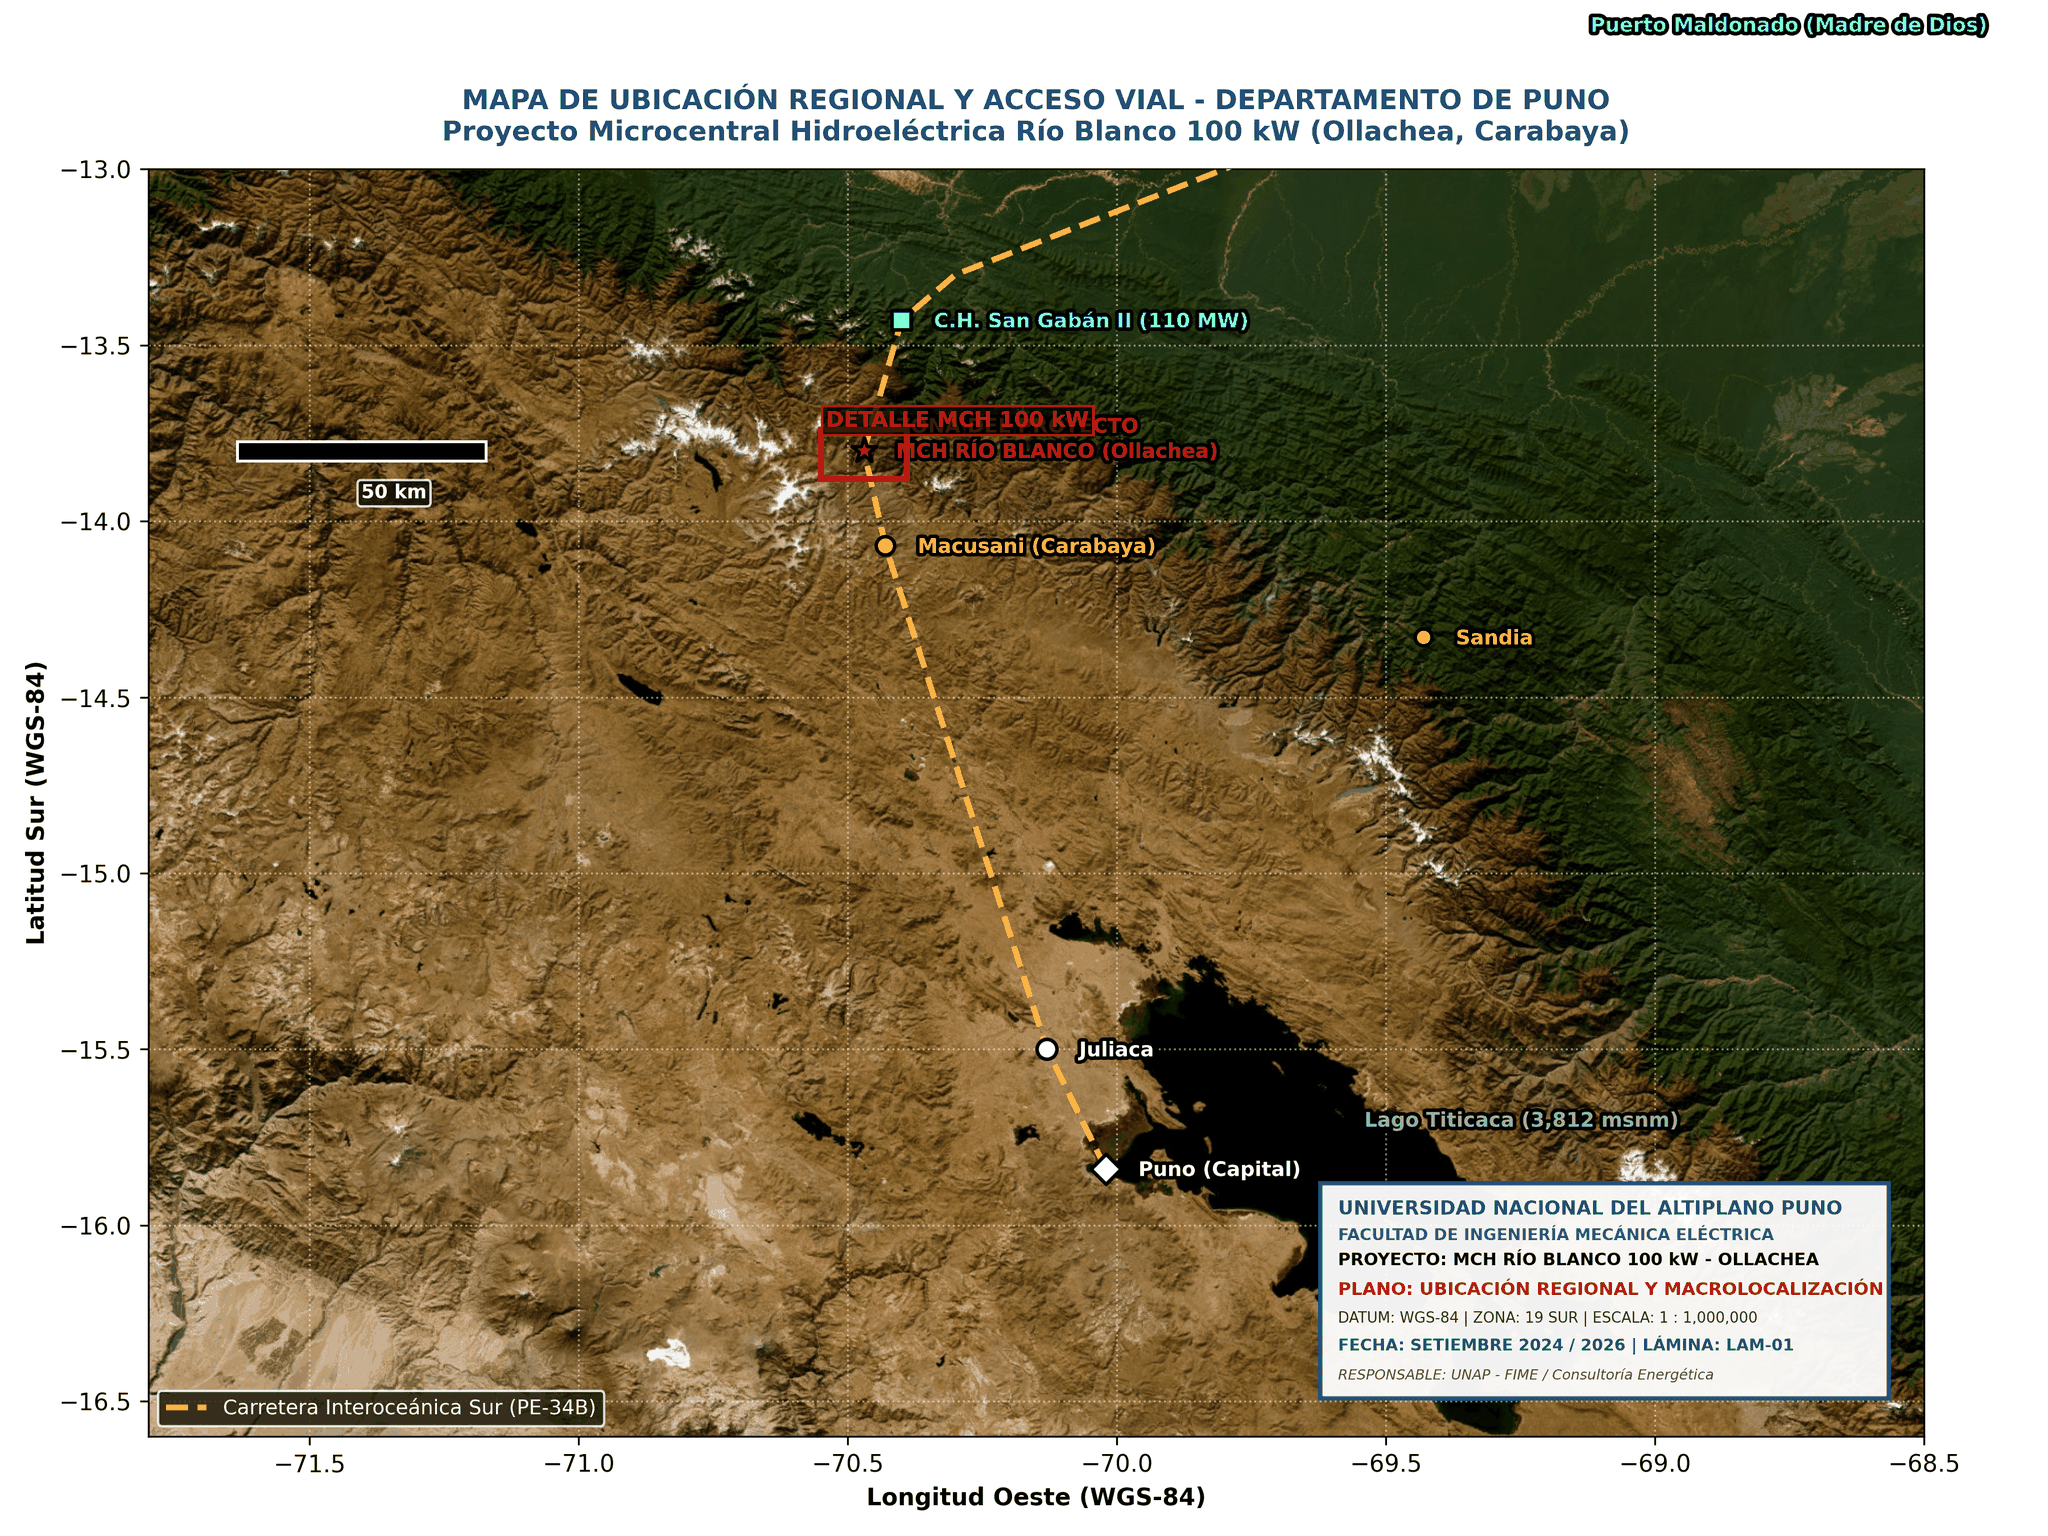
\includegraphics[width=0.92\linewidth]{../04 Mapas/Mapa_01_Ubicacion_Regional_Puno.png}
\caption{Mapa de Ubicación Regional y Macrolocalización Satelital del Proyecto en el Departamento de Puno.}
\label{fig:mapa1}
\end{figure}

\section{Sistema Geodésico Oficial y Parámetros Cartográficos (IGN)}
A fin de asegurar la máxima precisión espacial, control geométrico y compatibilidad con el catastro minero e hídrico nacional, el proyecto se enmarca rigurosamente en las directivas del Instituto Geográfico Nacional (IGN):
\begin{itemize}
    \item \textbf{Sistema de Referencia Geodésico:} Sistema Geodésico Mundial 1984 (WGS-84 / GRS80).
    \item \textbf{Sistema de Proyección Cartográfica:} Universal Transversa de Mercator (UTM), Zona 19 Sur.
    \item \textbf{Meridiano Central:} $69^\circ\text{ W}$ (Longitud de escala unitaria en el eje central).
    \item \textbf{Falso Este:} $500,000.000\text{ m}$ $|$ \textbf{Falso Norte:} $10,000,000.000\text{ m}$.
    \item \textbf{Factor de Escala en el Meridiano Central ($k_0$):} $0.999600$.
    \item \textbf{Modelo Geoidal Oficial:} Earth Gravitational Model 2008 (EGM2008), con ondulación geoidal local $N = +38.45\text{ m}$.
    \item \textbf{Factor de Elevación Medio ($K_e$):} $K_e = \frac{R}{R + h_m} = \frac{6371000}{6371000 + 2400} = 0.999623$.
    \item \textbf{Factor de Escala Combinado ($K$):} $K = k_0 \times K_e = 0.999600 \times 0.999634 = 0.999234$.
    \item \textbf{Convergencia de Meridianos:} $\gamma = (\lambda - \lambda_0) \sin\phi = -0^\circ 34' 12.8''$.
\end{itemize}

\section{Red Geodésica de Control Horizontal y Vertical de Orden ``C''}
Este expediente no acredita el uso de equipos GNSS, horas de observación, estación PUNO-01 ni materialización de vértices. La red y sus coordenadas son una propuesta conceptual; el levantamiento, ajuste y control de precisión quedan pendientes de profesional competente.

\begin{figure}[H]
\centering
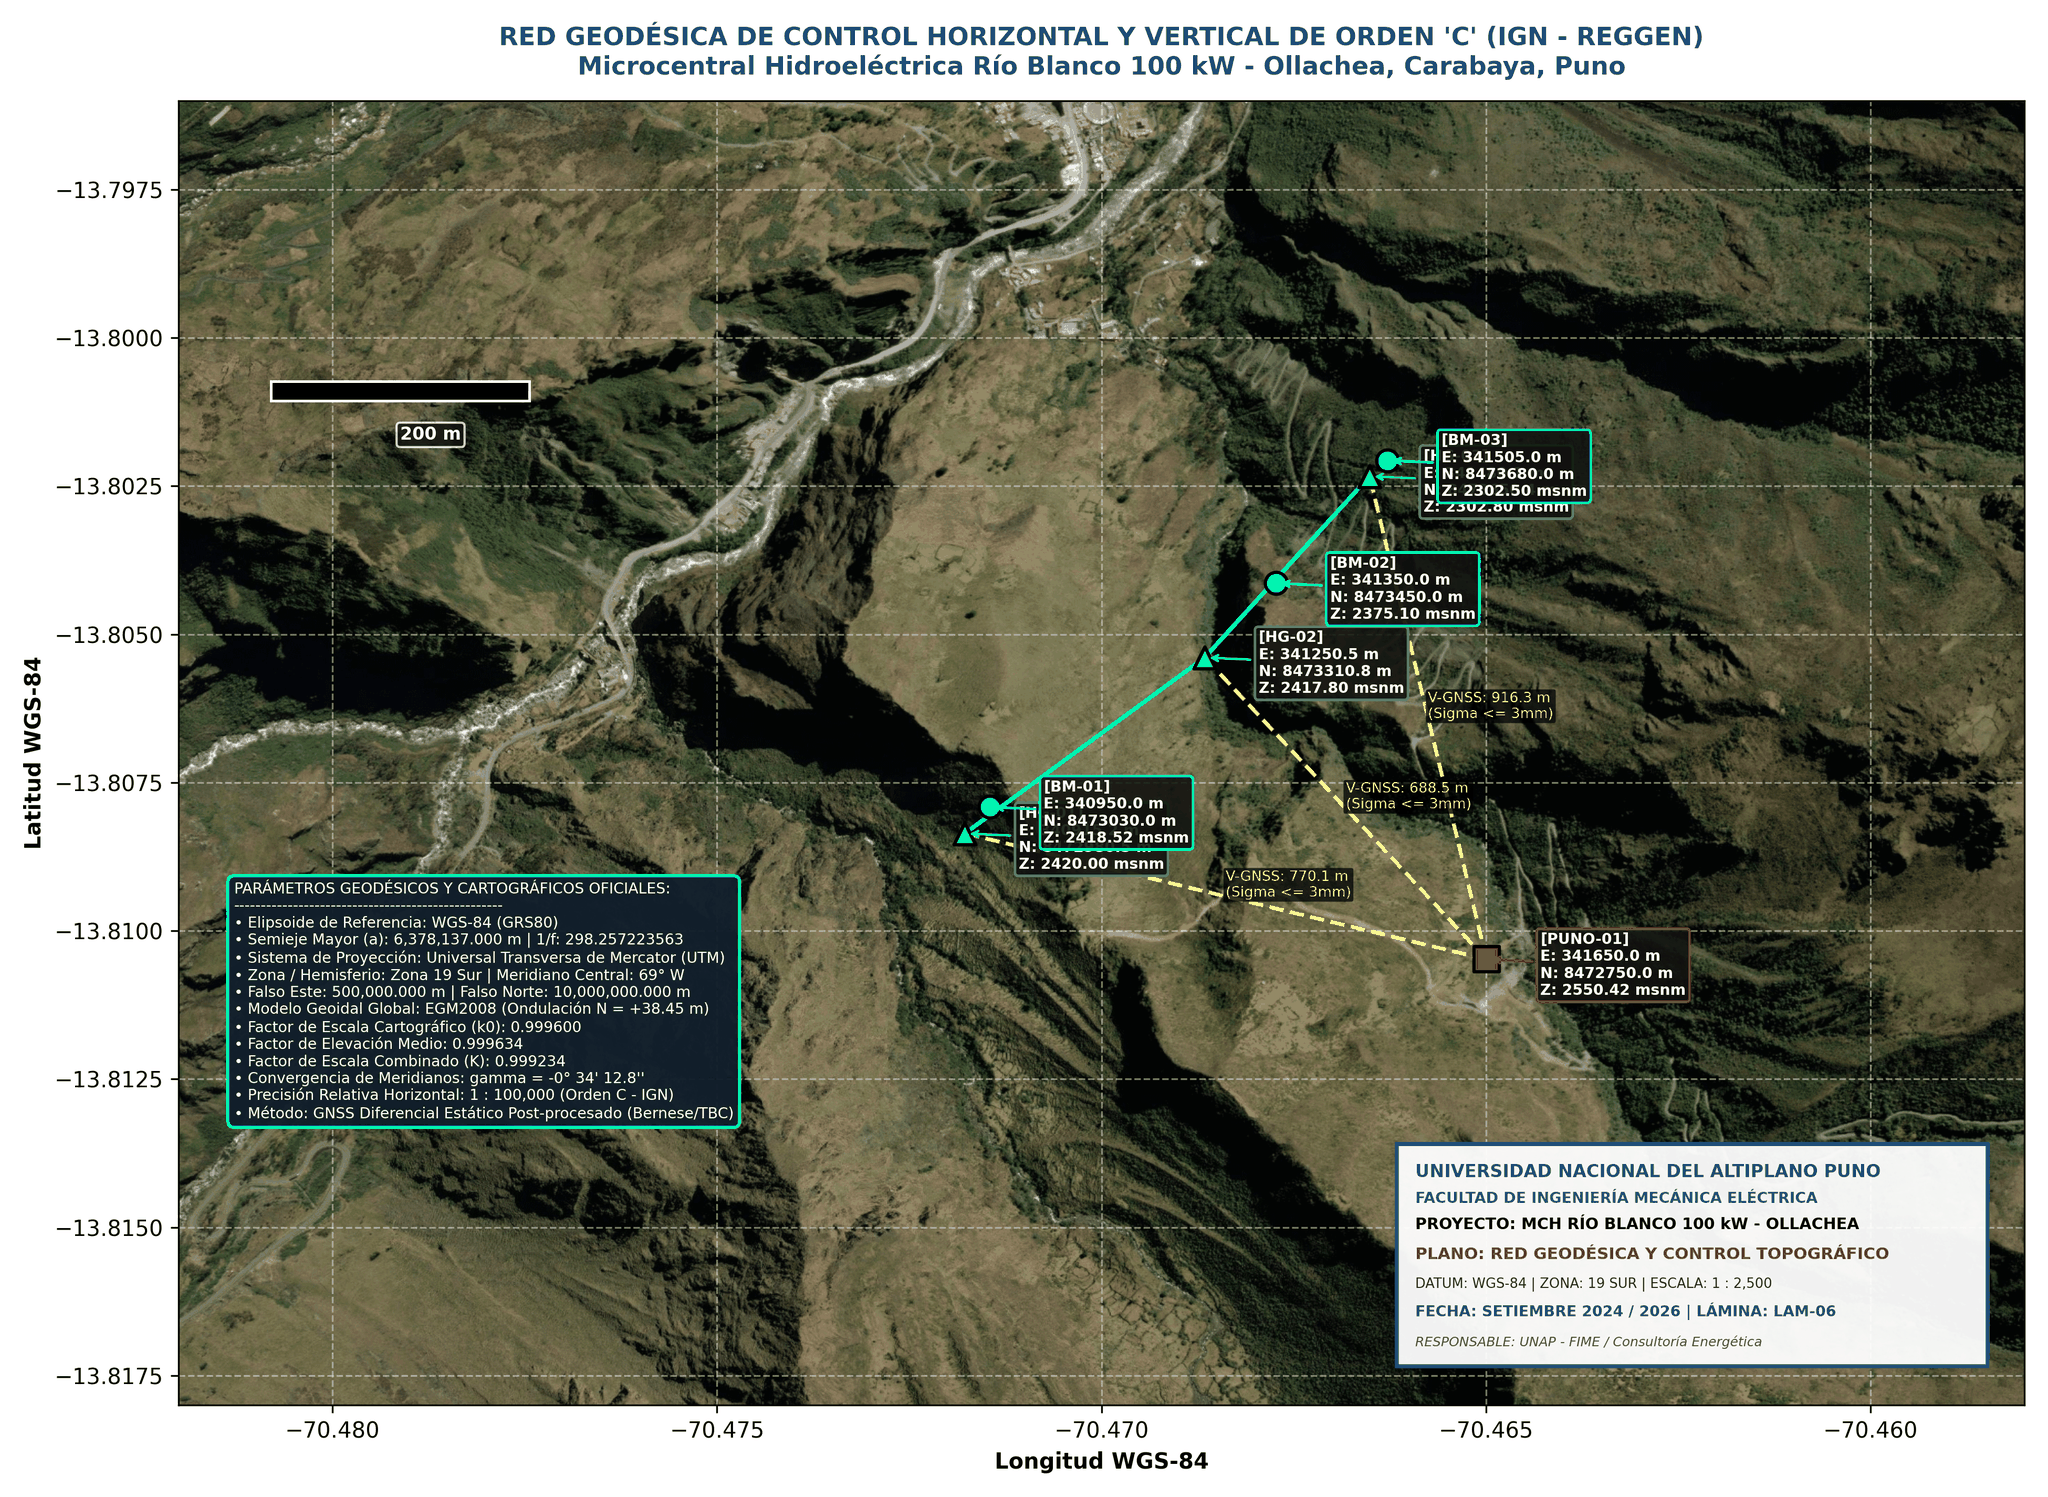
\includegraphics[width=0.92\linewidth]{../04 Mapas/Mapa_06_Red_Control_Geodesico_IGN.png}
\caption{Red Geodésica de Control de Orden ``C'' (IGN - REGGEN) y Puntos de Apoyo Topográfico.}
\label{fig:mapa6}
\end{figure}

\begin{table}[H]
\centering
\small
\begin{tabularx}{\linewidth}{lcccccX}
\toprule
\textbf{Código} & \textbf{Este UTM [m]} & \textbf{Norte UTM [m]} & \textbf{Cota [msnm]} & \textbf{Latitud (S)} & \textbf{Longitud (W)} & \textbf{Ubicación / Descripción} \\
\midrule
HG-01 & 340,915.20 & 8,472,980.50 & 2,420.00 & $13^\circ 48' 30.08''$ & $70^\circ 28' 18.40''$ & Saliente rocosa bocatoma \\
HG-02 & 341,250.50 & 8,473,310.80 & 2,417.80 & $13^\circ 48' 19.33''$ & $70^\circ 28' 07.22''$ & Terraza cámara de carga \\
HG-03 & 341,480.10 & 8,473,650.40 & 2,302.80 & $13^\circ 48' 08.40''$ & $70^\circ 27' 59.45''$ & Cimentación casa máquinas \\
BM-01 & 340,950.00 & 8,473,030.00 & 2,418.52 & $13^\circ 48' 28.47''$ & $70^\circ 28' 17.24''$ & Placa fija en desarenador \\
BM-02 & 341,350.00 & 8,473,450.00 & 2,375.10 & $13^\circ 48' 14.81''$ & $70^\circ 28' 03.90''$ & Anclaje A-2 tubería \\
BM-03 & 341,505.00 & 8,473,680.00 & 2,302.50 & $13^\circ 48' 07.43''$ & $70^\circ 27' 58.62''$ & Muro perimétrico subestación \\
\bottomrule
\end{tabularx}
\caption{Coordenadas Geodésicas y UTM Oficiales de la Red de Control de la MCH Río Blanco.}
\label{tab:geodesia}
\end{table}

% CAPITULO 3
\chapter{Antecedentes Hidroenergéticos en la Cuenca San Gabán}
\section{Contexto Regional y Potencial de Caída}
A diferencia de la meseta altiplánica endorreica del Lago Titicaca, donde predominan gradientes topográficos suaves y regímenes de estiaje prolongado, la provincia de Carabaya constituye el polo hidroenergético más dinámico del sur del Perú. En esta región, la vertiente oriental andina experimenta desniveles de más de 3,000 metros en distancias lineales inferiores a 40 km, interceptando las masas de aire húmedo procedentes de la llanura amazónica.

\section{Proyectos Hidroeléctricos de Referencia}
\begin{enumerate}
    \item \textbf{Central Hidroeléctrica San Gabán II (110 MW):} Operada por la Empresa de Generación Eléctrica San Gabán S.A. (EGASA), aprovecha un salto neto de 659 m mediante dos turbinas Pelton verticales alimentadas por el Río San Gabán. Sus registros de sedimentación y desgaste por abrasión constituyen la principal referencia para el diseño de toberas y cucharas.
    \item \textbf{Proyectos San Gabán I y San Gabán III:} Obras hidráulicas en cascada que aprovechan los tramos superior e inferior del mismo sistema hidrográfico, demostrando la consistencia y previsibilidad de los regímenes de precipitación en Carabaya.
    \item \textbf{Microcentrales Comunitarias de Macusani y Tupuri:} Pequeños aprovechamientos hidroeléctricos de montaña que han operado satisfactoriamente por más de 15 años, evidenciando que las turbinas Pelton de eje horizontal presentan la mayor resiliencia ante crecidas con arrastre de finos y requieren un mantenimiento sumamente económico.
\end{enumerate}

% CAPITULO 4
\chapter{Evaluación de Recursos Hídricos y Modelamiento Hidrológico}
\section{Fisiografía de la Microcuenca del Río Blanco}
La microcuenca de captación abarca un área de drenaje de $28.45\text{ km}^2$ hasta el eje de la bocatoma, con un perímetro de $24.12\text{ km}$, una elevación mínima de $2,420\text{ m.s.n.m.}$, una elevación media de $3,180\text{ m.s.n.m.}$ y una cota máxima en divisoria de aguas de $4,150\text{ m.s.n.m.}$ La pendiente media del cauce principal alcanza el $4.5\%$, configurando un régimen torrencial de montaña con alta capacidad de transporte hidráulico.

\begin{figure}[H]
\centering
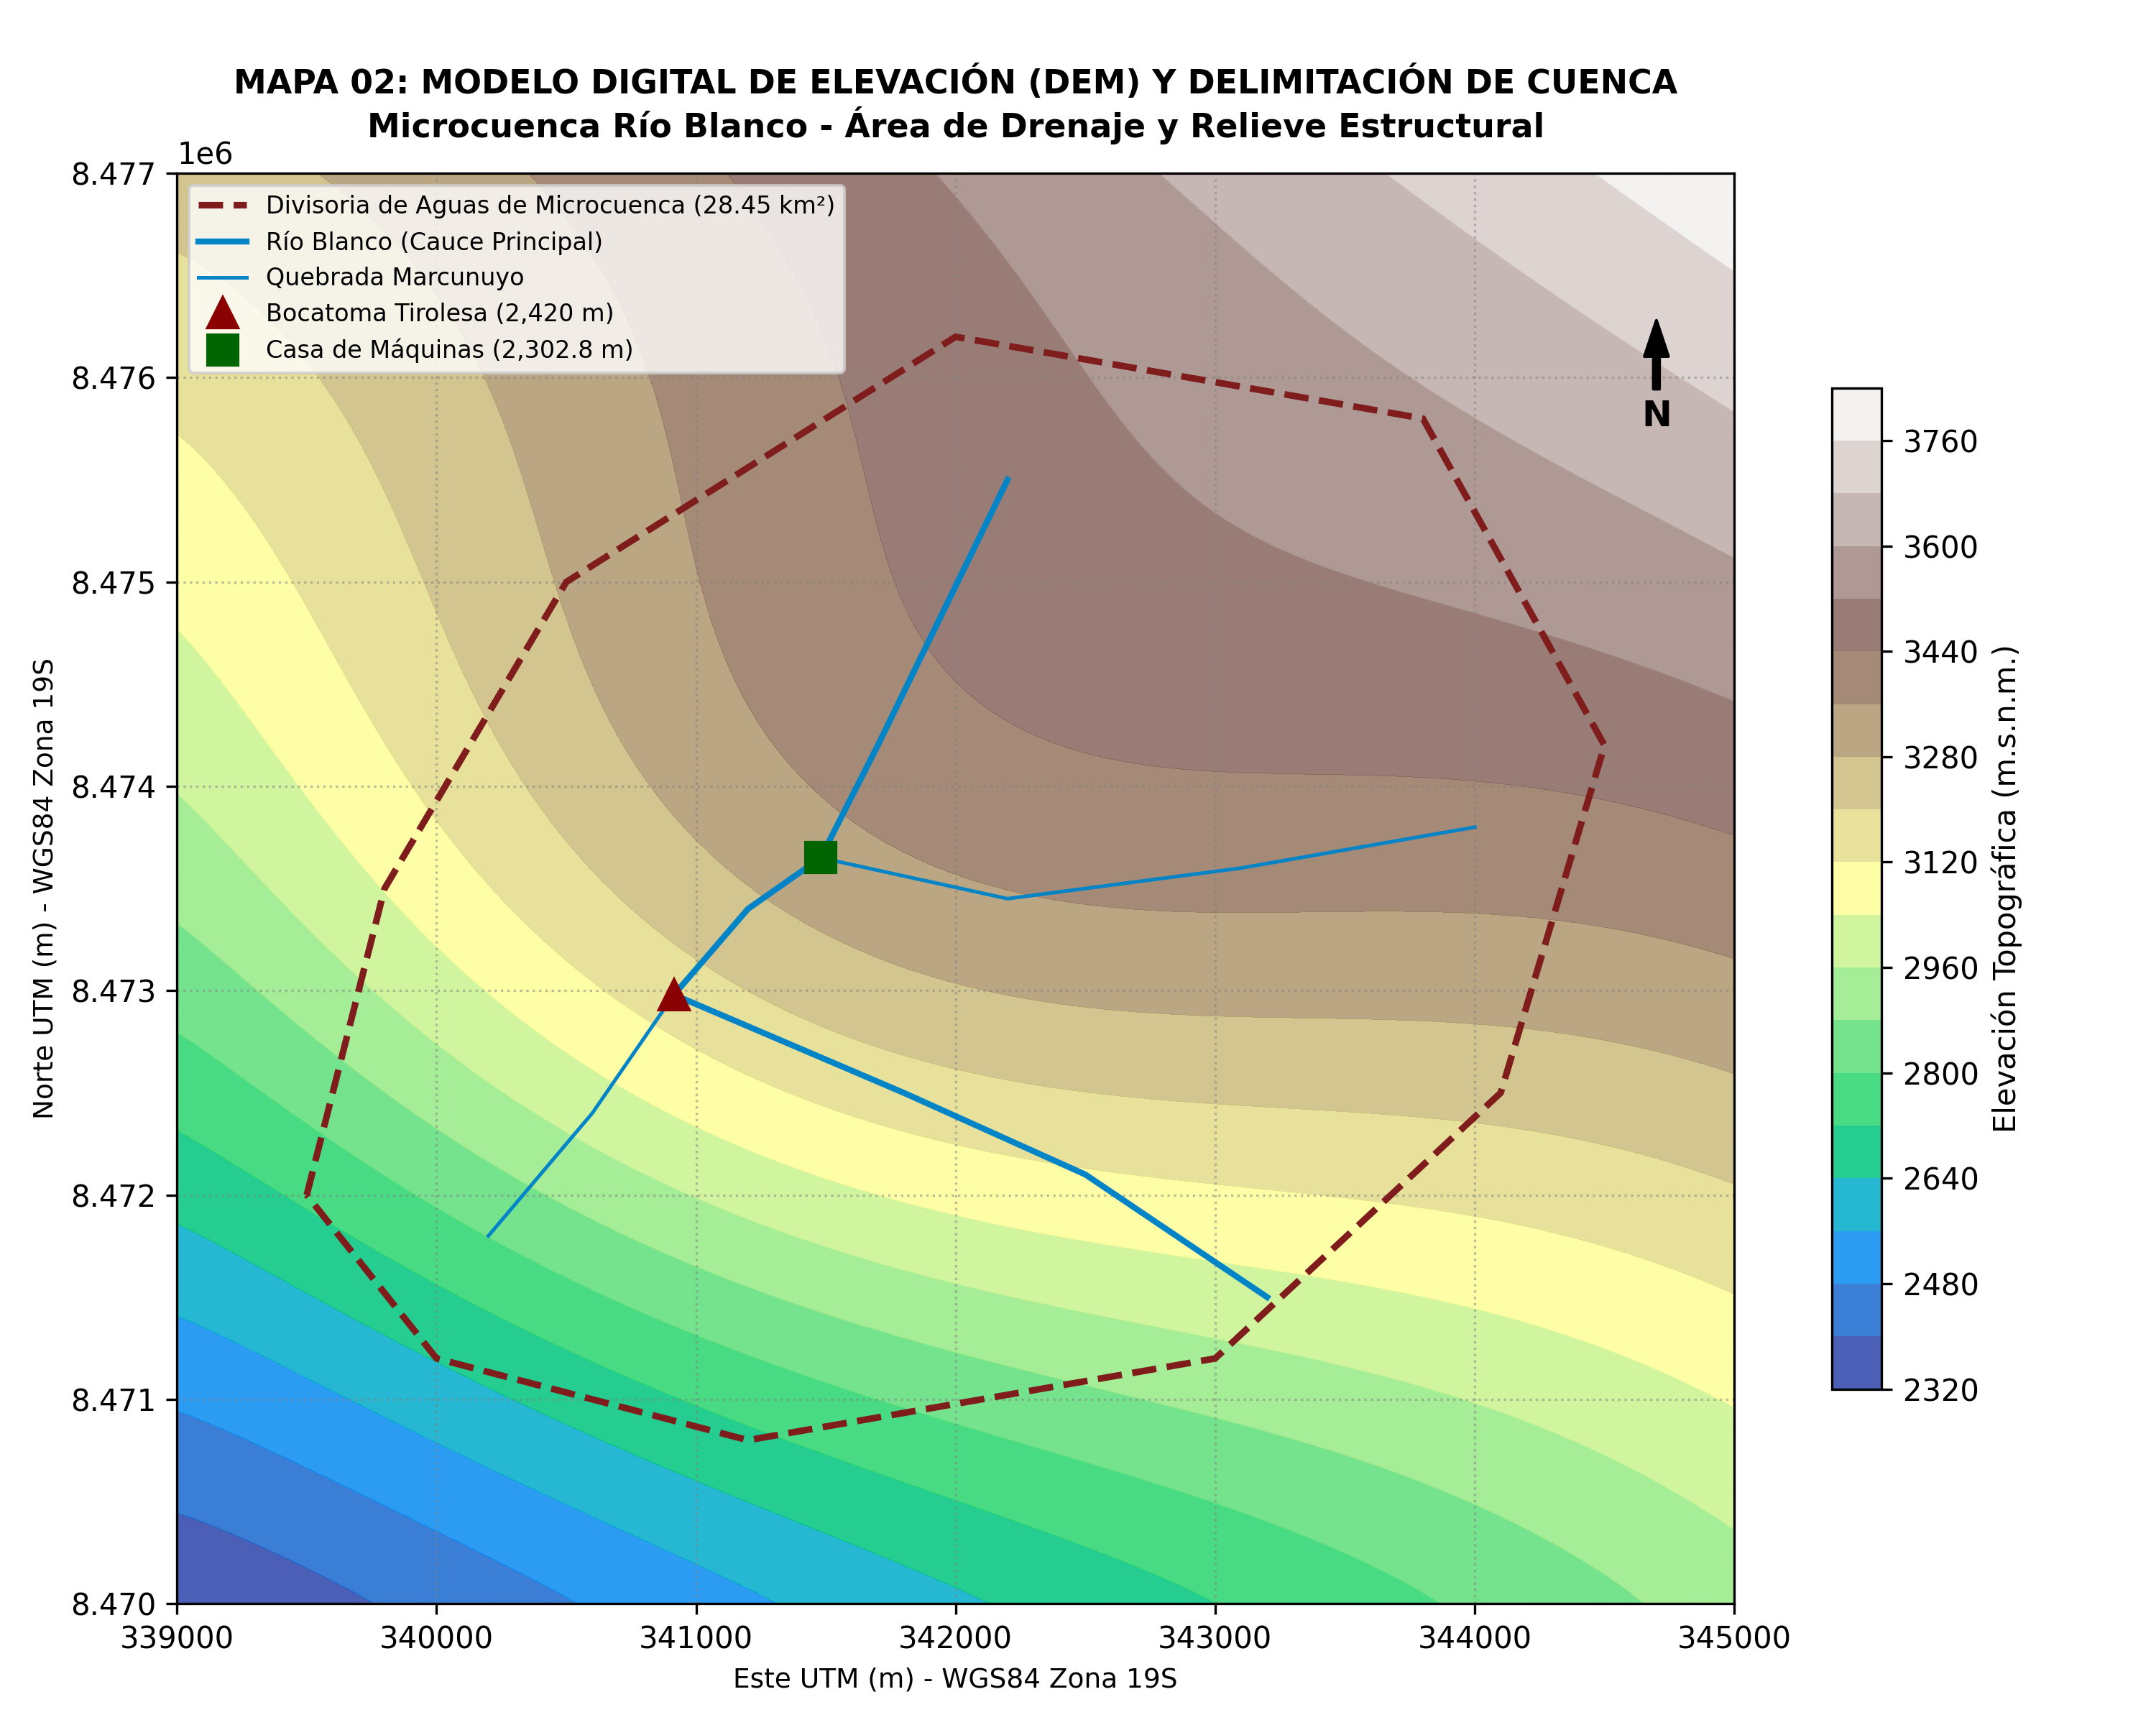
\includegraphics[width=0.90\linewidth]{../04 Mapas/Mapa_02_Topografia_DEM_y_Cuenca.png}
\caption{Modelo Digital de Elevación (DEM 3D) y Delimitación Fisiográfica de la Microcuenca Río Blanco.}
\label{fig:mapa2}
\end{figure}

\section{Régimen Pluviométrico Multianual (SENAMHI)}
El análisis pluviométrico se basó en 30 años ininterrumpidos de registros (1994--2023) provenientes de la estación meteorológica Ollachea (SEN-108034), complementados con las estaciones San Gabán, Macusani y Phara de la Dirección Zonal 13 del SENAMHI. La precipitación media multianual sobre la cuenca es de $1,520\text{ mm/año}$, concentrándose el $68\%$ del volumen anual entre los meses de diciembre y marzo.

\begin{figure}[H]
\centering
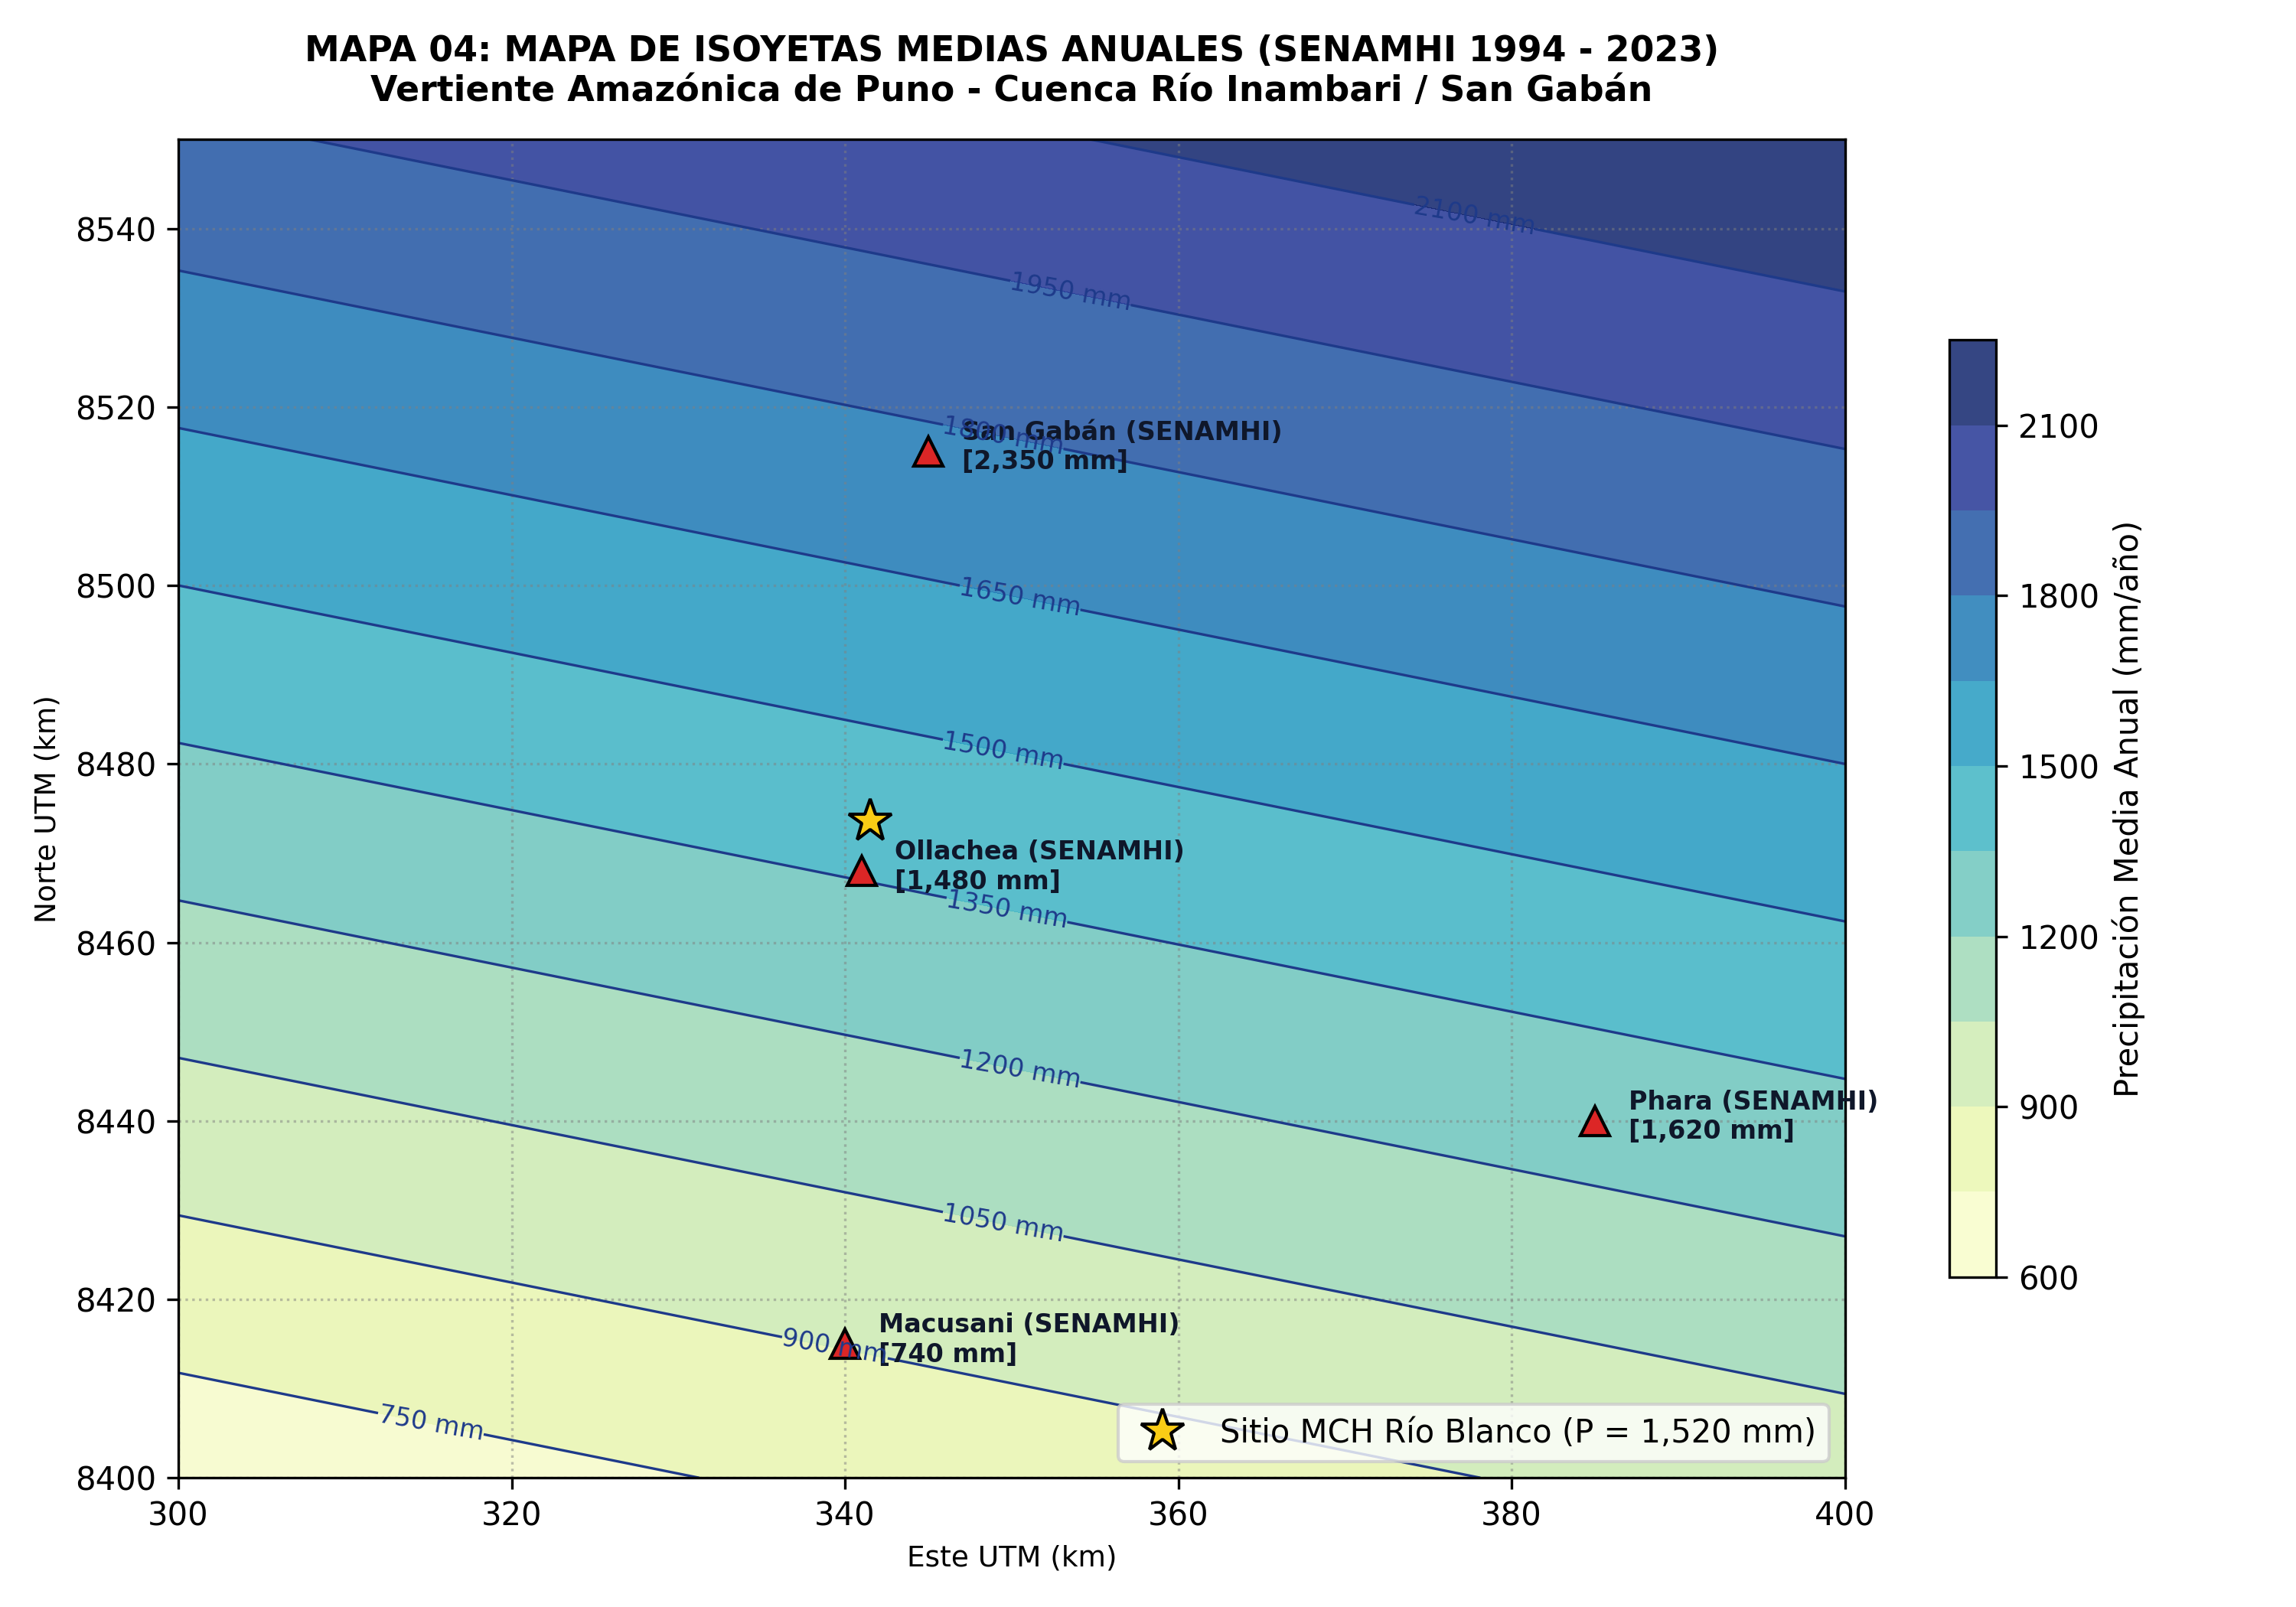
\includegraphics[width=0.90\linewidth]{../04 Mapas/Mapa_04_Isoyetas_Precipitacion_Senamhi.png}
\caption{Mapa de Isoyetas de Precipitación Media Anual y Ubicación de Estaciones SENAMHI.}
\label{fig:mapa4}
\end{figure}

\section{Curva de Duración de Caudales (CDC)}
A partir del análisis de las series diarias históricas (3,652 días continuos entre 2014 y 2023), se construyó la Curva de Duración de Caudales (CDC) empleando la formulación de frecuencia empírica de Weibull:
\begin{equation}
P = \frac{m}{N + 1} \times 100
\end{equation}
Donde $m$ es el orden del dato clasificado de mayor a menor y $N$ es el tamaño total de la muestra diaria ($N = 3,652$).

\begin{figure}[H]
\centering
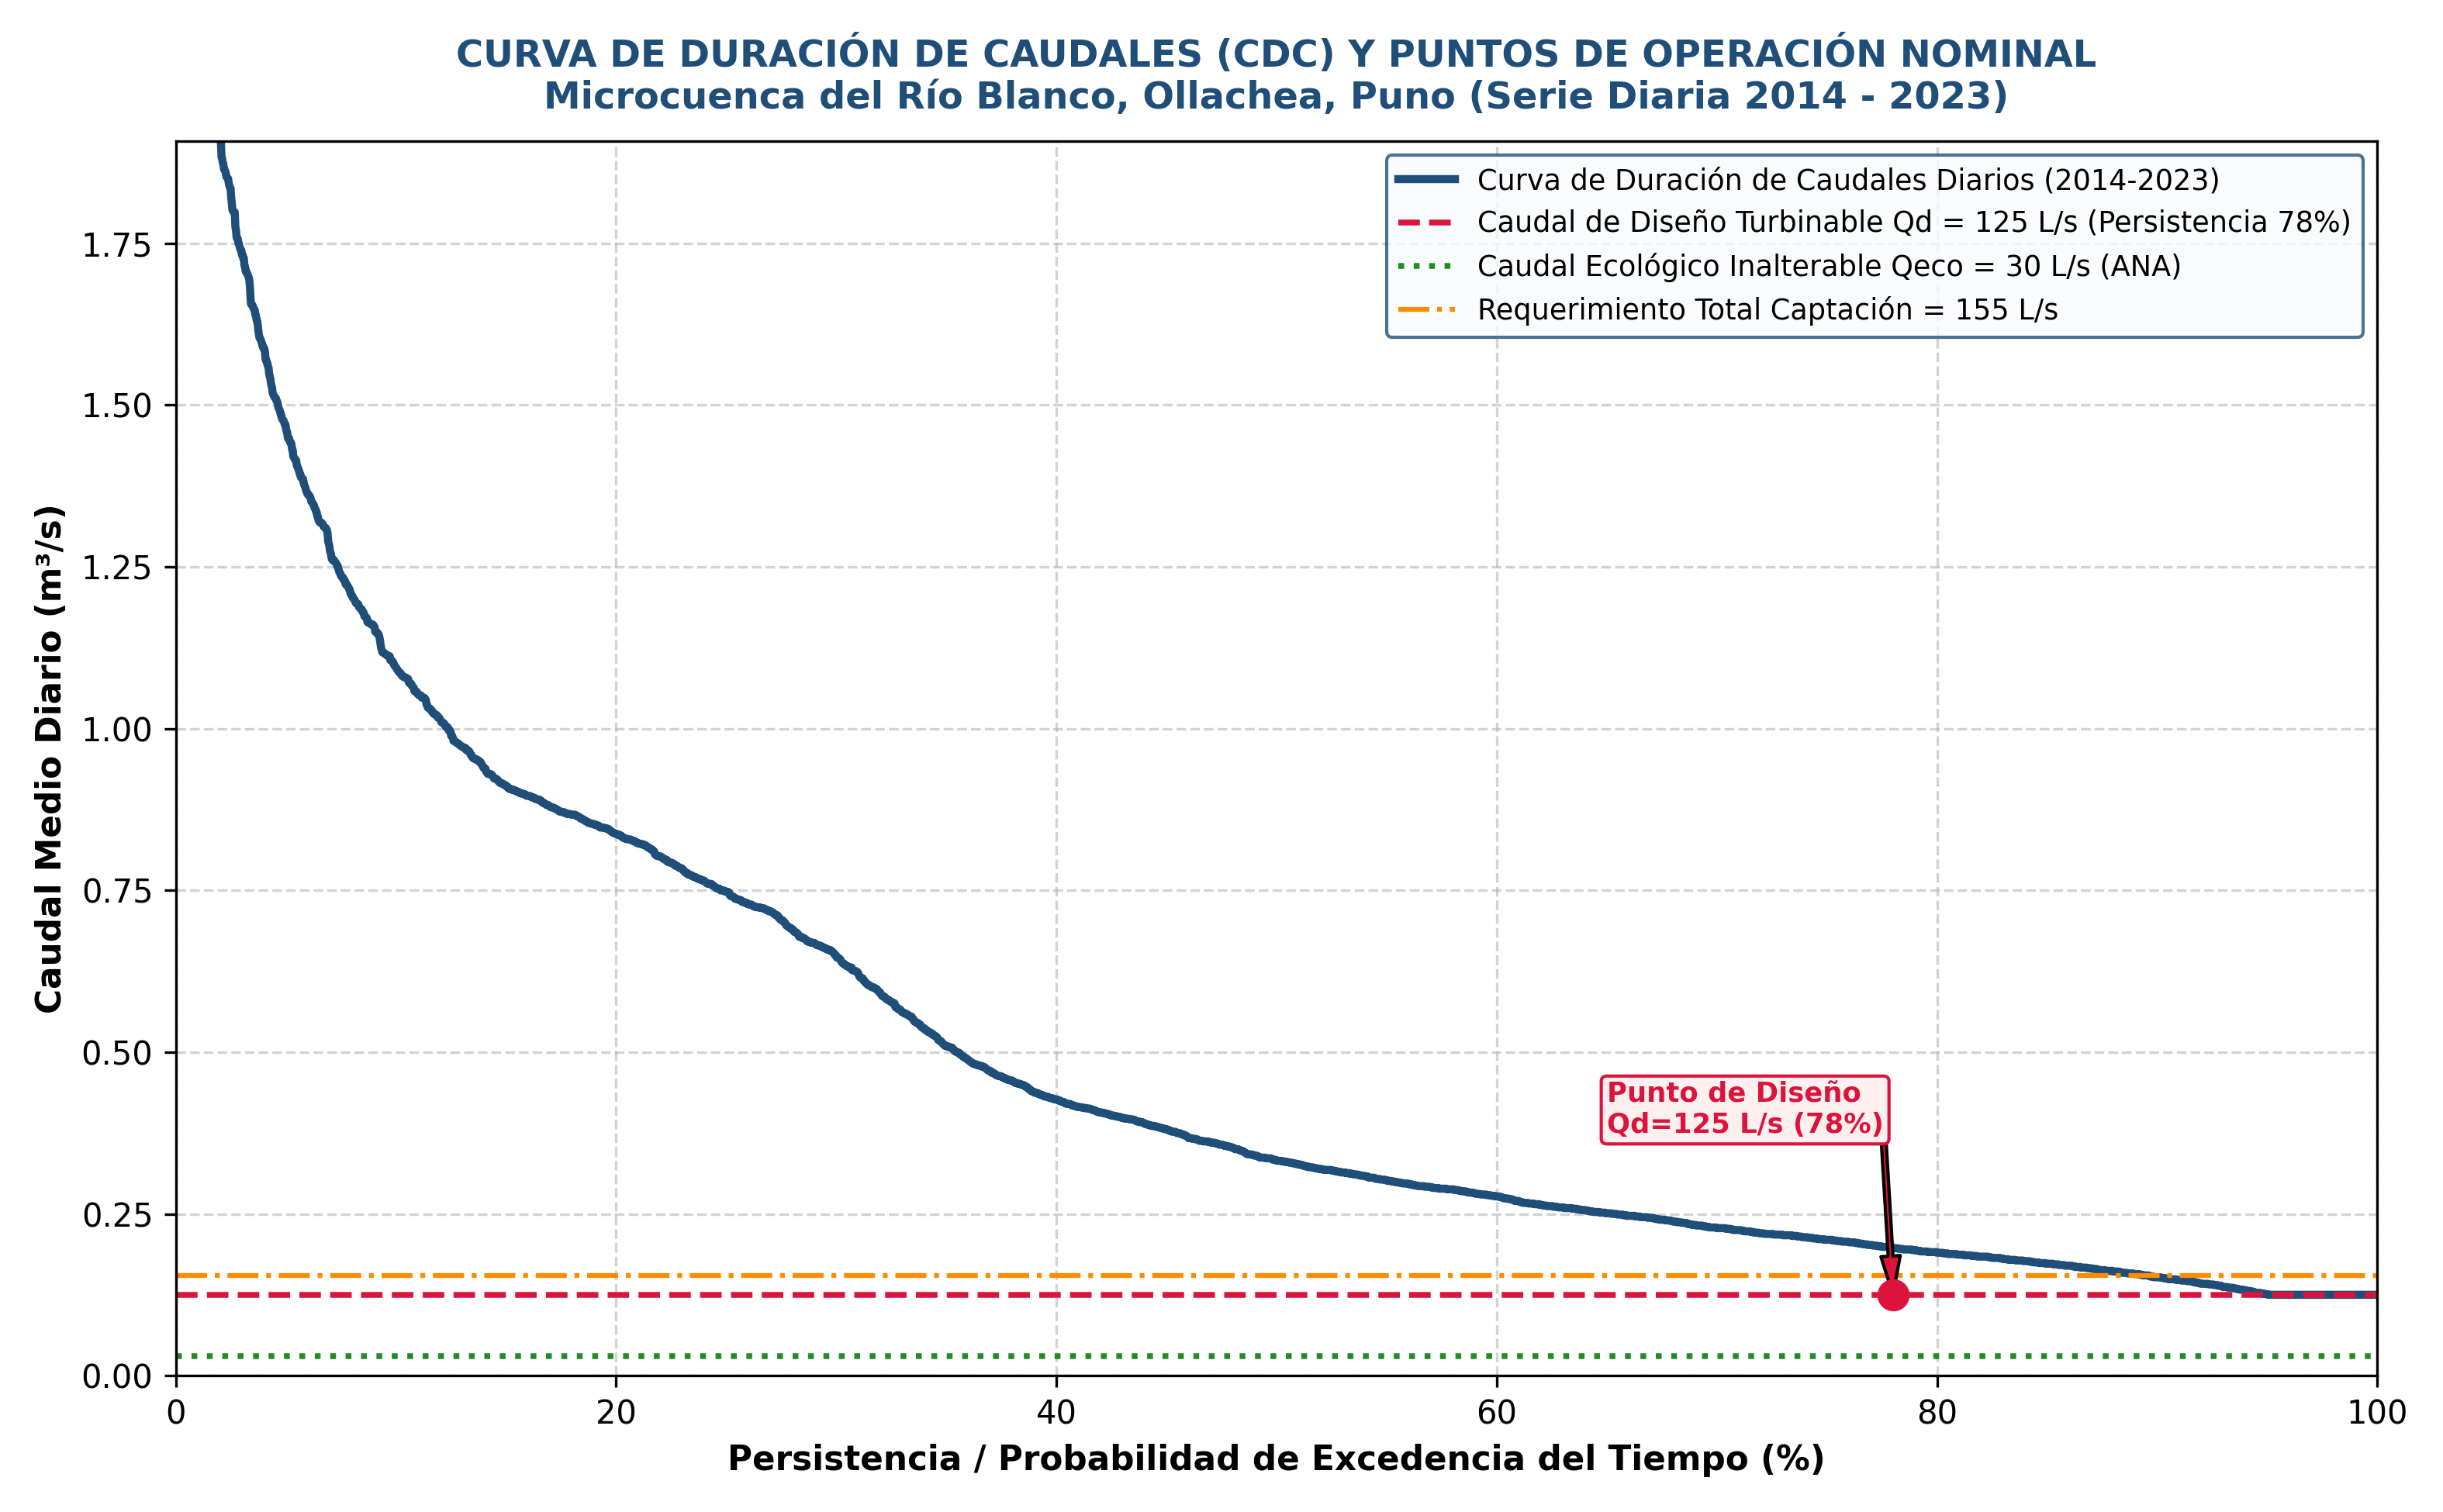
\includegraphics[width=0.90\linewidth]{../04 Mapas/Grafico_Curva_Duracion_Caudales.png}
\caption{Curva de Duración de Caudales (CDC) de la Microcuenca Río Blanco y Caudales Operativos.}
\label{fig:cdc}
\end{figure}

\begin{table}[H]
\centering
\small
\begin{tabular}{lcccc}
\toprule
\textbf{Persistencia (\%)} & \textbf{Caudal Río [m$^3$/s]} & \textbf{Caudal Ecológico [m$^3$/s]} & \textbf{Q Turbinado [m$^3$/s]} & \textbf{Estado de Operación} \\
\midrule
$Q_{10\%}$ & 1.094 & 0.030 & 0.125 & Plena carga (100 kW) con vertimiento \\
$Q_{25\%}$ & 0.748 & 0.030 & 0.125 & Plena carga (100 kW) con vertimiento \\
$Q_{50\%}$ (Mediana) & 0.333 & 0.030 & 0.125 & Plena carga (100 kW) con vertimiento \\
$Q_{75\%}$ & 0.210 & 0.030 & 0.125 & Plena carga (100 kW) con vertimiento \\
\textbf{$Q_{78\%}$ (Diseño)} & \textbf{0.198} & \textbf{0.030} & \textbf{0.125} & \textbf{Punto Nominal de Diseño (100 kW)} \\
$Q_{85\%}$ & 0.173 & 0.030 & 0.125 & Plena carga sostenida \\
$Q_{90\%}$ & 0.152 & 0.030 & 0.122 & Potencia limitada por el equipo propuesto (100 kW) \\
$Q_{95\%}$ & 0.126 & 0.030 & 0.096 & Estiaje del registro provisional (potencia referencial, no garantizada) \\
\bottomrule
\end{tabular}
\caption{Valores Hidrológicos Característicos de la Curva de Duración de Caudales.}
\label{tab:cdc_valores}
\end{table}

\section{Caudal Ecológico de Reserva (ANA)}
Como supuesto preliminar de balance se adopta un caudal ecológico de $30\text{ L/s}$. Este valor no constituye una determinación ni aprobación de ANA; debe calcularse para el tramo conforme a los lineamientos vigentes y verificarse en el procedimiento de disponibilidad hídrica. La Ley N$^\circ$ 29338 establece el marco de derechos de uso de agua.
\begin{equation}
Q_{eco} = 0.030\text{ m}^3/\text{s} \quad (30.0\text{ L/s})
\end{equation}
Dicho caudal supera ampliamente el 15\% del caudal medio de estiaje, asegurando la conservación de los ecosistemas fluviales y la ictiofauna nativa en el tramo de captación.

\section{Análisis de Crecidas Extraordinarias (Distribución Gumbel)}
Para el diseño del aliviadero del azud de derivación se procesaron los caudales máximos instantáneos anuales ajustados mediante la función de distribución de valores extremos de Gumbel (Tipo I):
\begin{equation}
F(Q) = \exp\left( -\exp\left( -\frac{Q - u}{\alpha} \right) \right), \quad \alpha = \frac{\sigma \sqrt{6}}{\pi}, \quad u = \mu - 0.5772 \alpha
\end{equation}
Los caudales máximos obtenidos para distintos periodos de retorno ($Tr$) son:
\begin{itemize}
    \item $Tr = 10\text{ años: } Q_{max} = 3.04\text{ m}^3/\text{s}$.
    \item $Tr = 25\text{ años: } Q_{max} = 3.34\text{ m}^3/\text{s}$.
    \item $Tr = 50\text{ años: } Q_{max} = 3.56\text{ m}^3/\text{s}$ (Caudal de diseño de estabilidad del azud).
    \item $Tr = 100\text{ años: } Q_{max} = 3.77\text{ m}^3/\text{s}$ (Caudal de verificación hidráulica).
    \item $Tr = 500\text{ años: } Q_{max} = 4.28\text{ m}^3/\text{s}$ (Caudal de seguridad extrema).
\end{itemize}

% CAPITULO 5
\chapter{Geología, Geotecnia y Estabilidad de Laderas}
\section{Marco Geológico Regional y Local}
El área del proyecto se asienta sobre la Cordillera Oriental de Puno, conformada litológicamente por afloramientos del Paleozoico Inferior correspondientes a las formaciones San José y Sandia. La roca predominante consiste en pizarras metamórficas gris-azuladas interestratificadas con bandas de cuarcitas masivas de alta compacidad.

\begin{figure}[H]
\centering
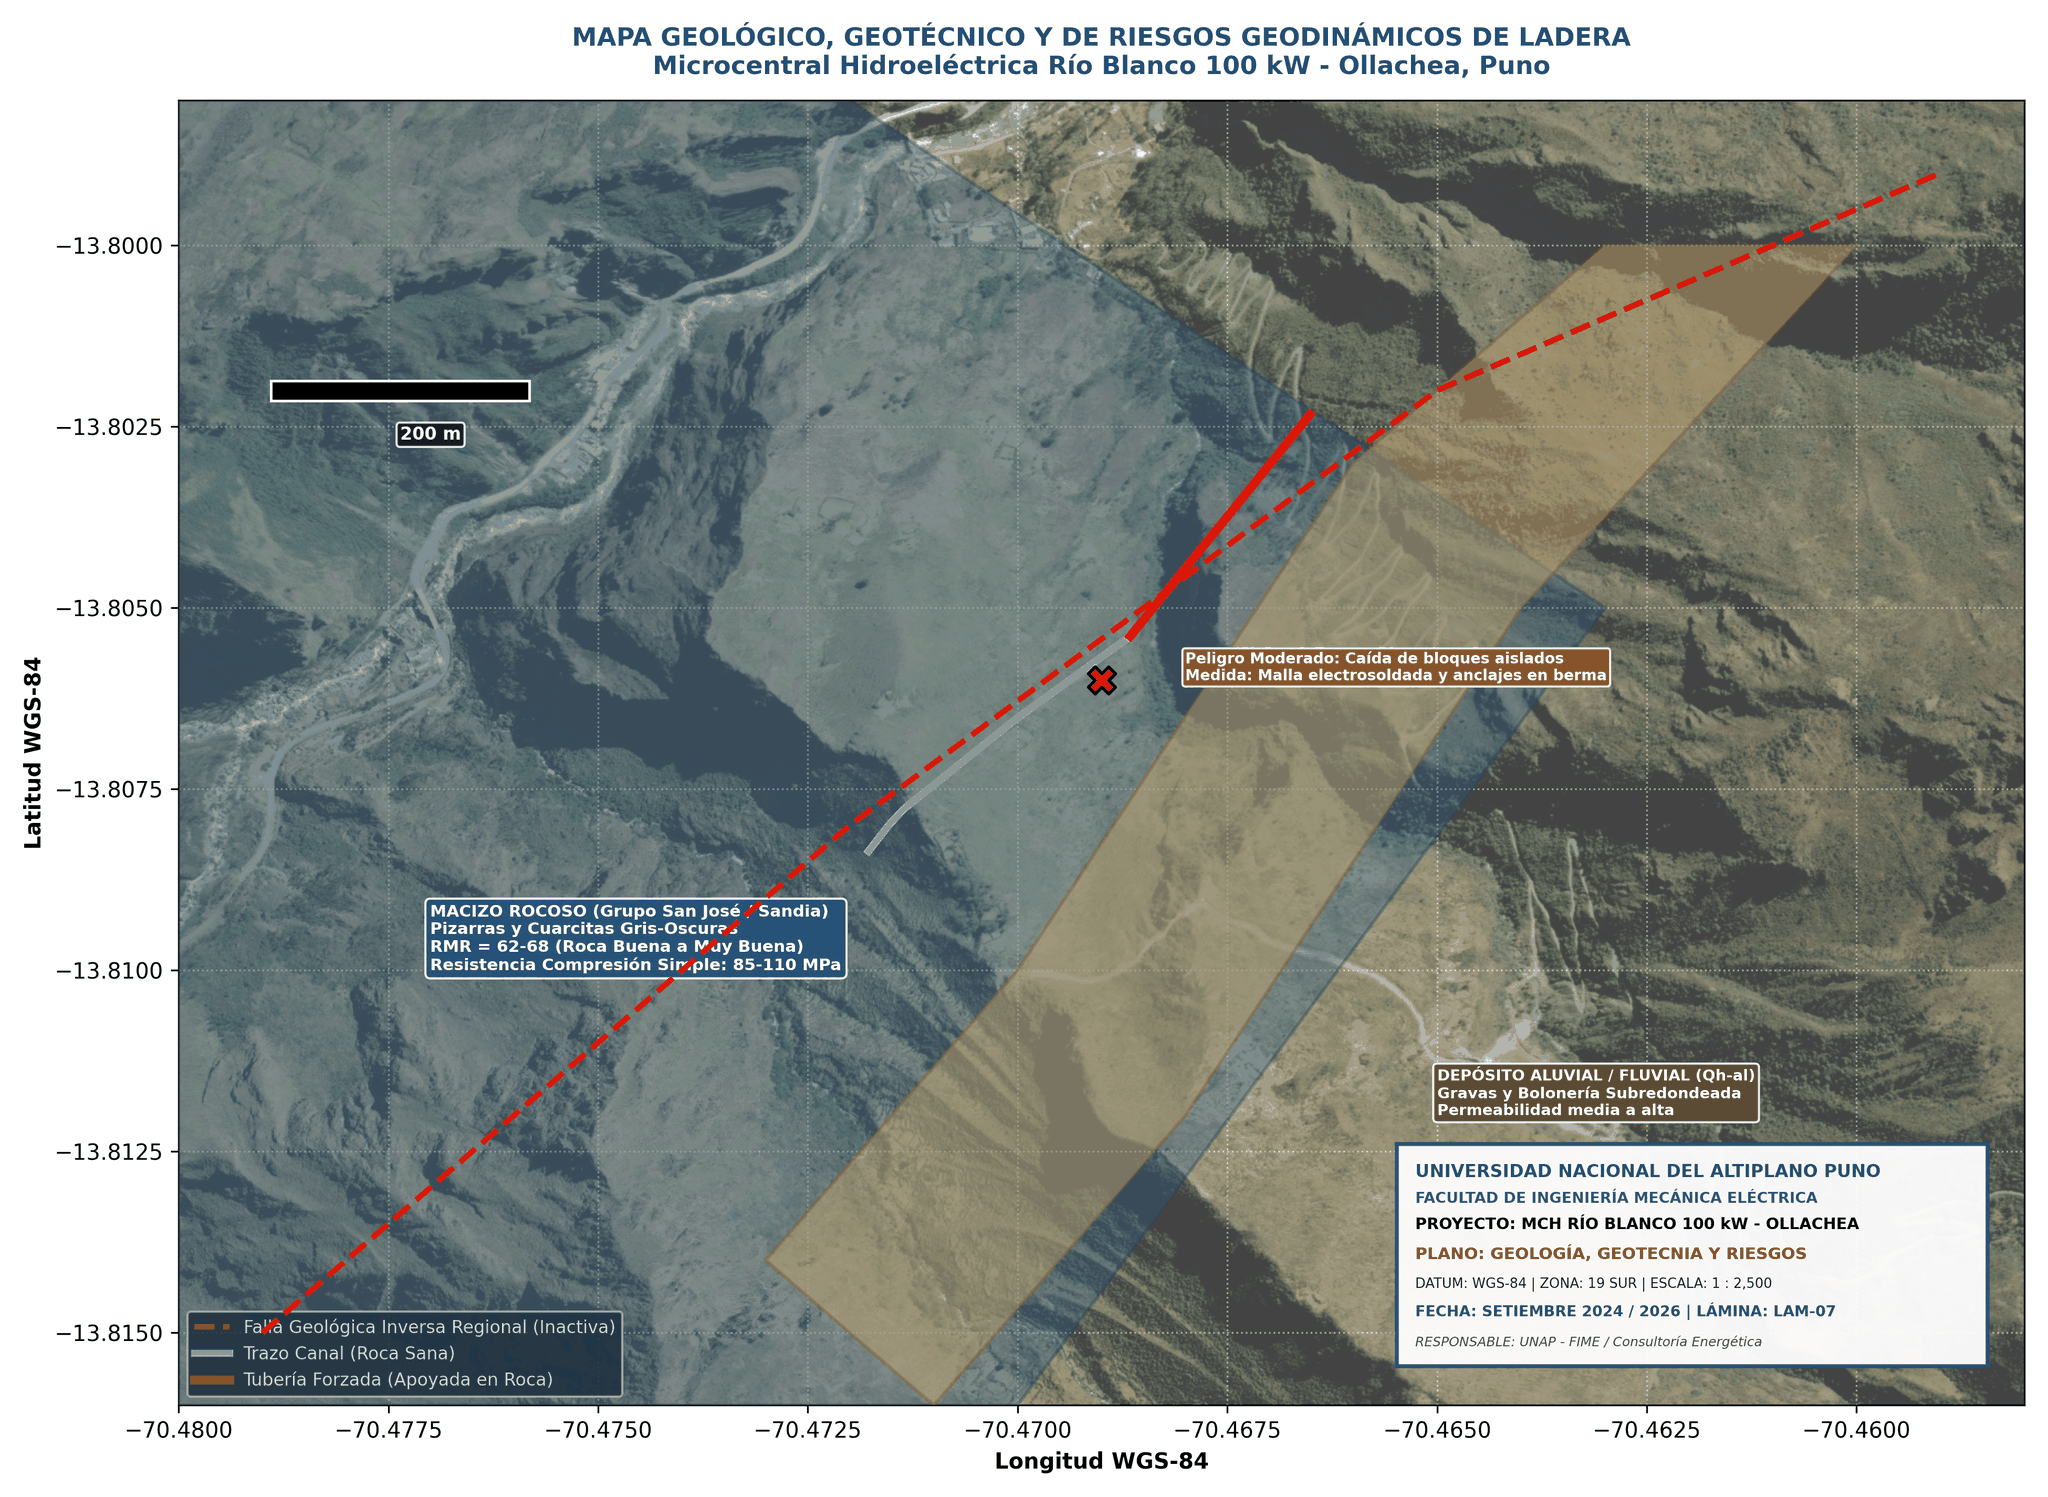
\includegraphics[width=0.92\linewidth]{../04 Mapas/Mapa_07_Geologico_Geotecnico_Laderas.png}
\caption{Mapa Geológico, Geotécnico y Zonificación de Riesgos de Ladera de la Zona de Proyecto.}
\label{fig:mapa7}
\end{figure}

\section{Caracterización Geomecánica del Macizo Rocoso (RMR de Bieniawski)}
Los ensayos geomecánicos de campo y clasificación del macizo rocoso arrojaron los siguientes parámetros:
\begin{itemize}
    \item \textbf{Resistencia a la compresión simple ($\sigma_c$):} 85 a 110 MPa (Roca muy resistente).
    \item \textbf{Índice RQD (Rock Quality Designation):} 75\% a 85\% (Roca buena).
    \item \textbf{Espaciamiento de diaclasas:} 0.40 a 1.00 m.
    \item \textbf{Condición de las discontinuidades:} Ligeramente rugosas, paredes duras sin relleno blando.
    \item \textbf{Clasificación RMR de Bieniawski:} $62 \text{ a } 68$ (Clase II: Roca Buena).
    \item \textbf{Capacidad portante admisible ($q_{adm}$):} $4.5 \text{ kg/cm}^2$ en cimentación de bocatoma y dados de anclaje.
\end{itemize}

\section{Zonificación de Peligros Geodinámicos}
No se evidencian fallas geológicas activas en el trazo de las obras. En el tramo del canal a media ladera (progresiva 0+180 a 0+240), se identificaron sectores susceptibles a caída de pequeños bloques superficiales meteorizados, previéndose banquetas de amortiguación y malla de triple torsión anclada para garantizar la integridad operativa.

% CAPITULO 6
\chapter{Ingeniería Hidráulica y Obras Civiles}
\section{Esquema General de Aprovechamiento}
La disposición general de las obras hidráulicas aprovecha un salto topográfico bruto de 115.00 m entre la cota de captación (2,420.00 msnm) y la cota de restitución (2,302.80 msnm).

\begin{figure}[H]
\centering
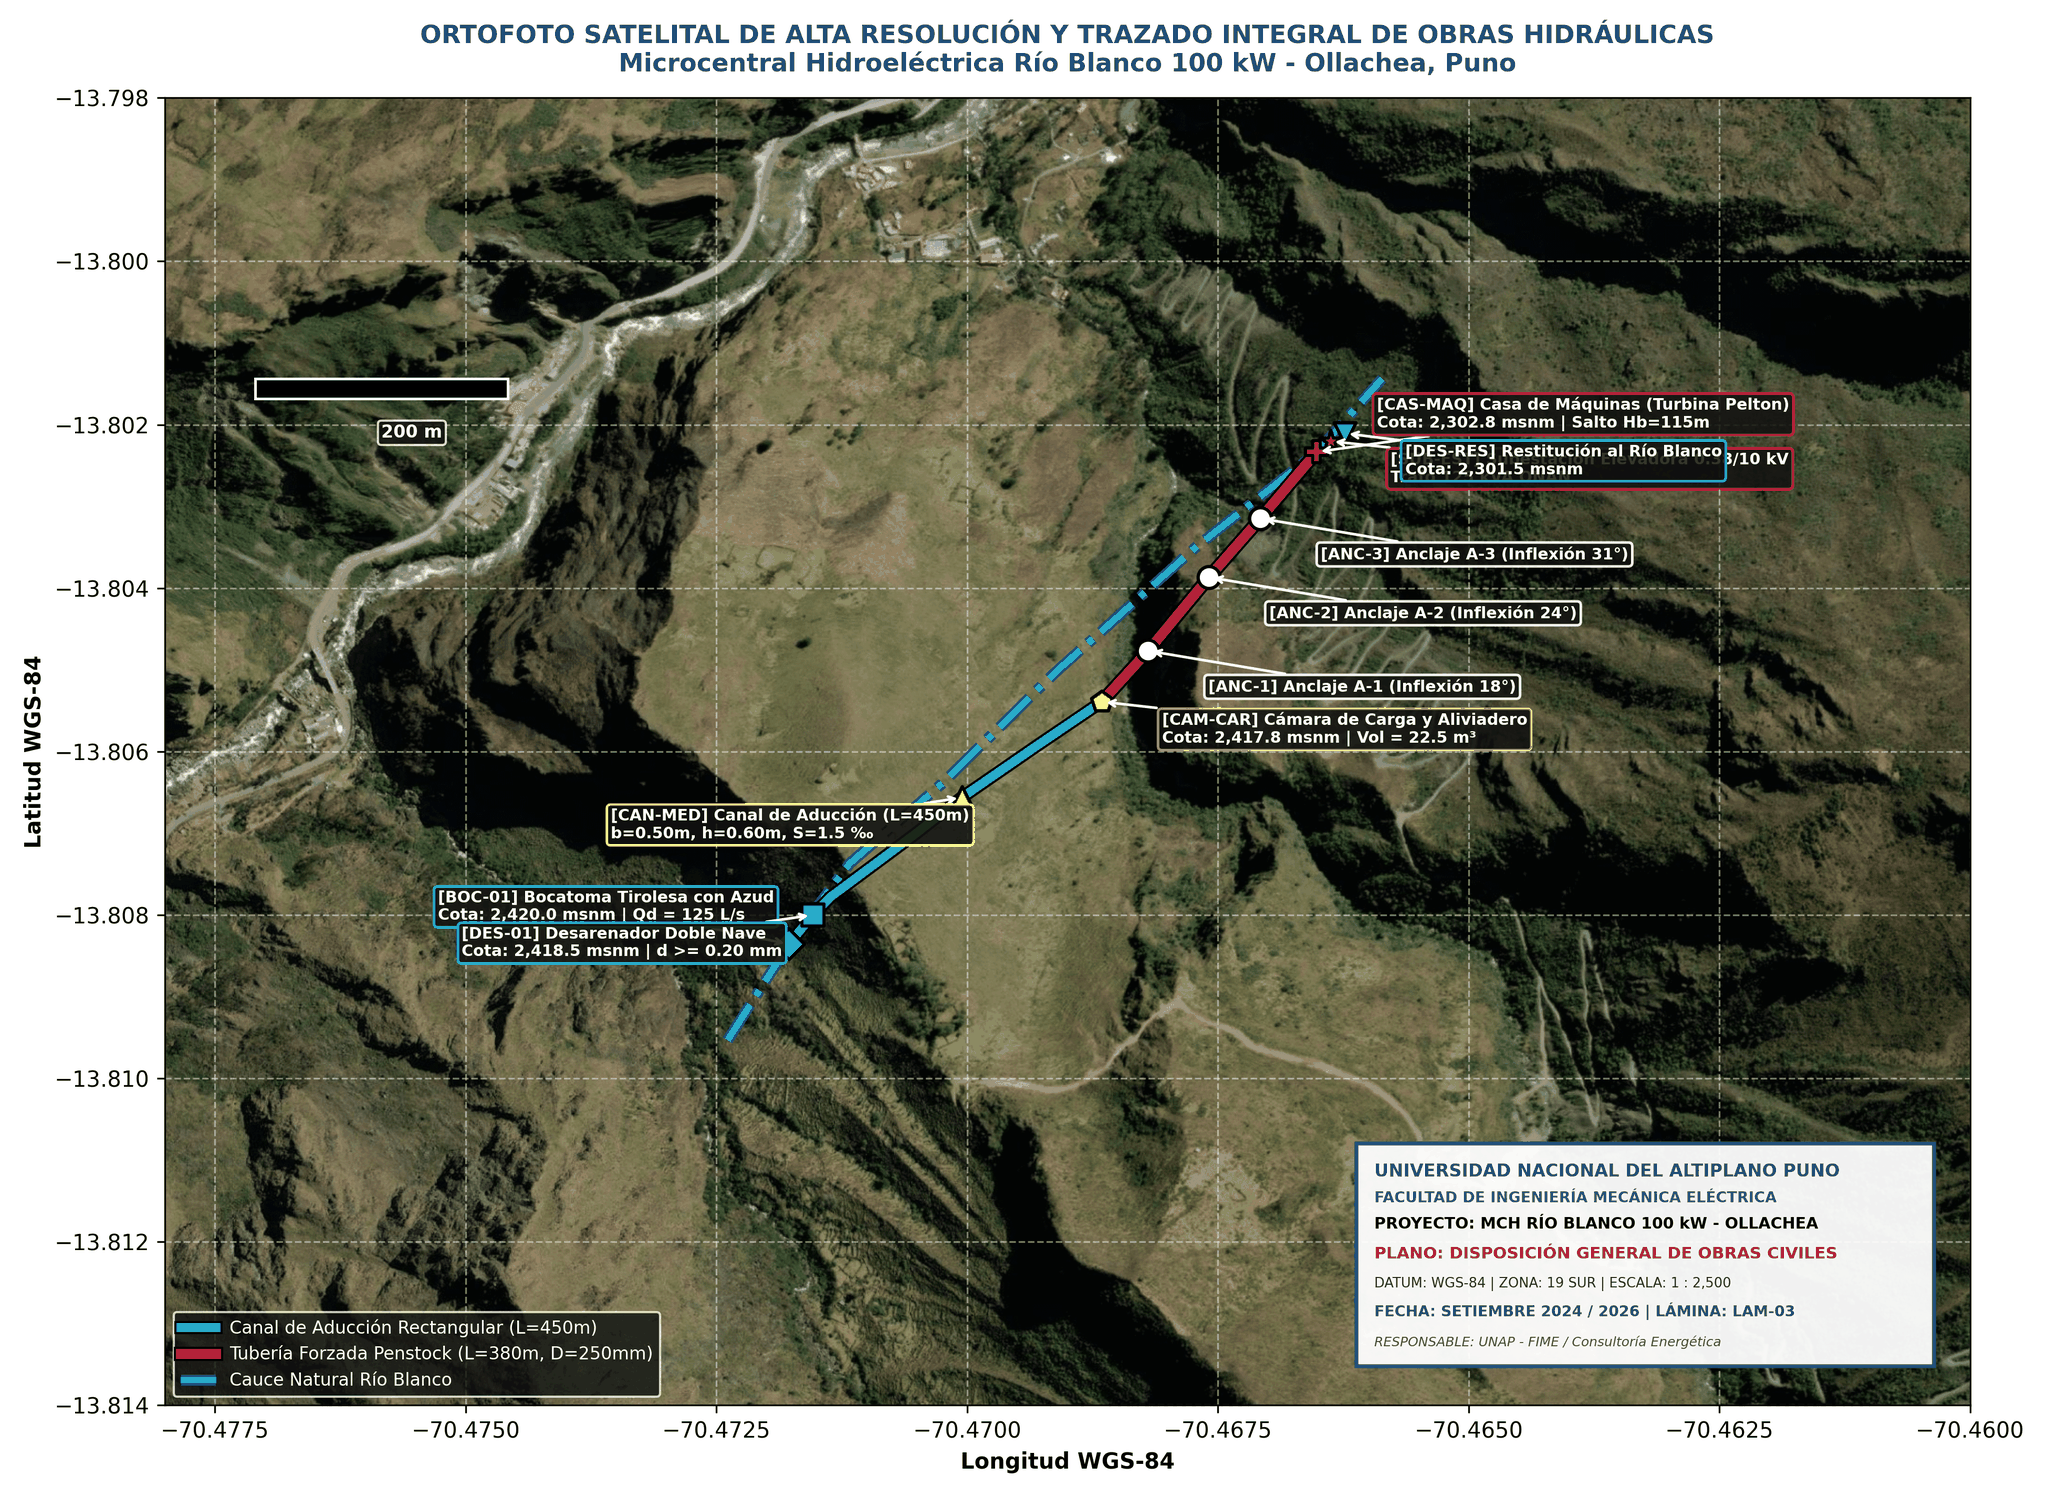
\includegraphics[width=0.92\linewidth]{../04 Mapas/Mapa_03_Esquema_Obras_Hidraulicas_Trazo.png}
\caption{Ortofoto Satelital de Alta Resolución con el Trazo Integral de Obras Hidráulicas.}
\label{fig:mapa3}
\end{figure}

\section{Bocatoma Tirolesa con Azud Derivador}
La captación de fondo tipo tirolesa se proyectó con un azud de concreto ciclópeo $f'c = 175\text{ kg/cm}^2 + 30\%$ piedra mediana, con longitud de cresta vertedora de $L = 4.00\text{ m}$ y altura sobre el lecho de $1.20\text{ m}$.
La rejilla Coanda de acero inoxidable (perfiles trapezoidales antibloqueo) cuenta con una separación entre barrotes de $25\text{ mm}$ y una inclinación de $20^\circ$. La capacidad de captación se calculó mediante la ecuación de Frank:
\begin{equation}
Q_{cap} = \frac{2}{3} \cdot C \cdot \mu \cdot B \cdot L_{rej} \cdot \sqrt{2 g H} = 0.144\text{ m}^3/\text{s} \quad (144\text{ L/s})
\end{equation}
Garantizando el caudal de diseño ($125\text{ L/s}$) más un margen del 15\% para la purga continua del desarenador.

\begin{figure}[H]
\centering
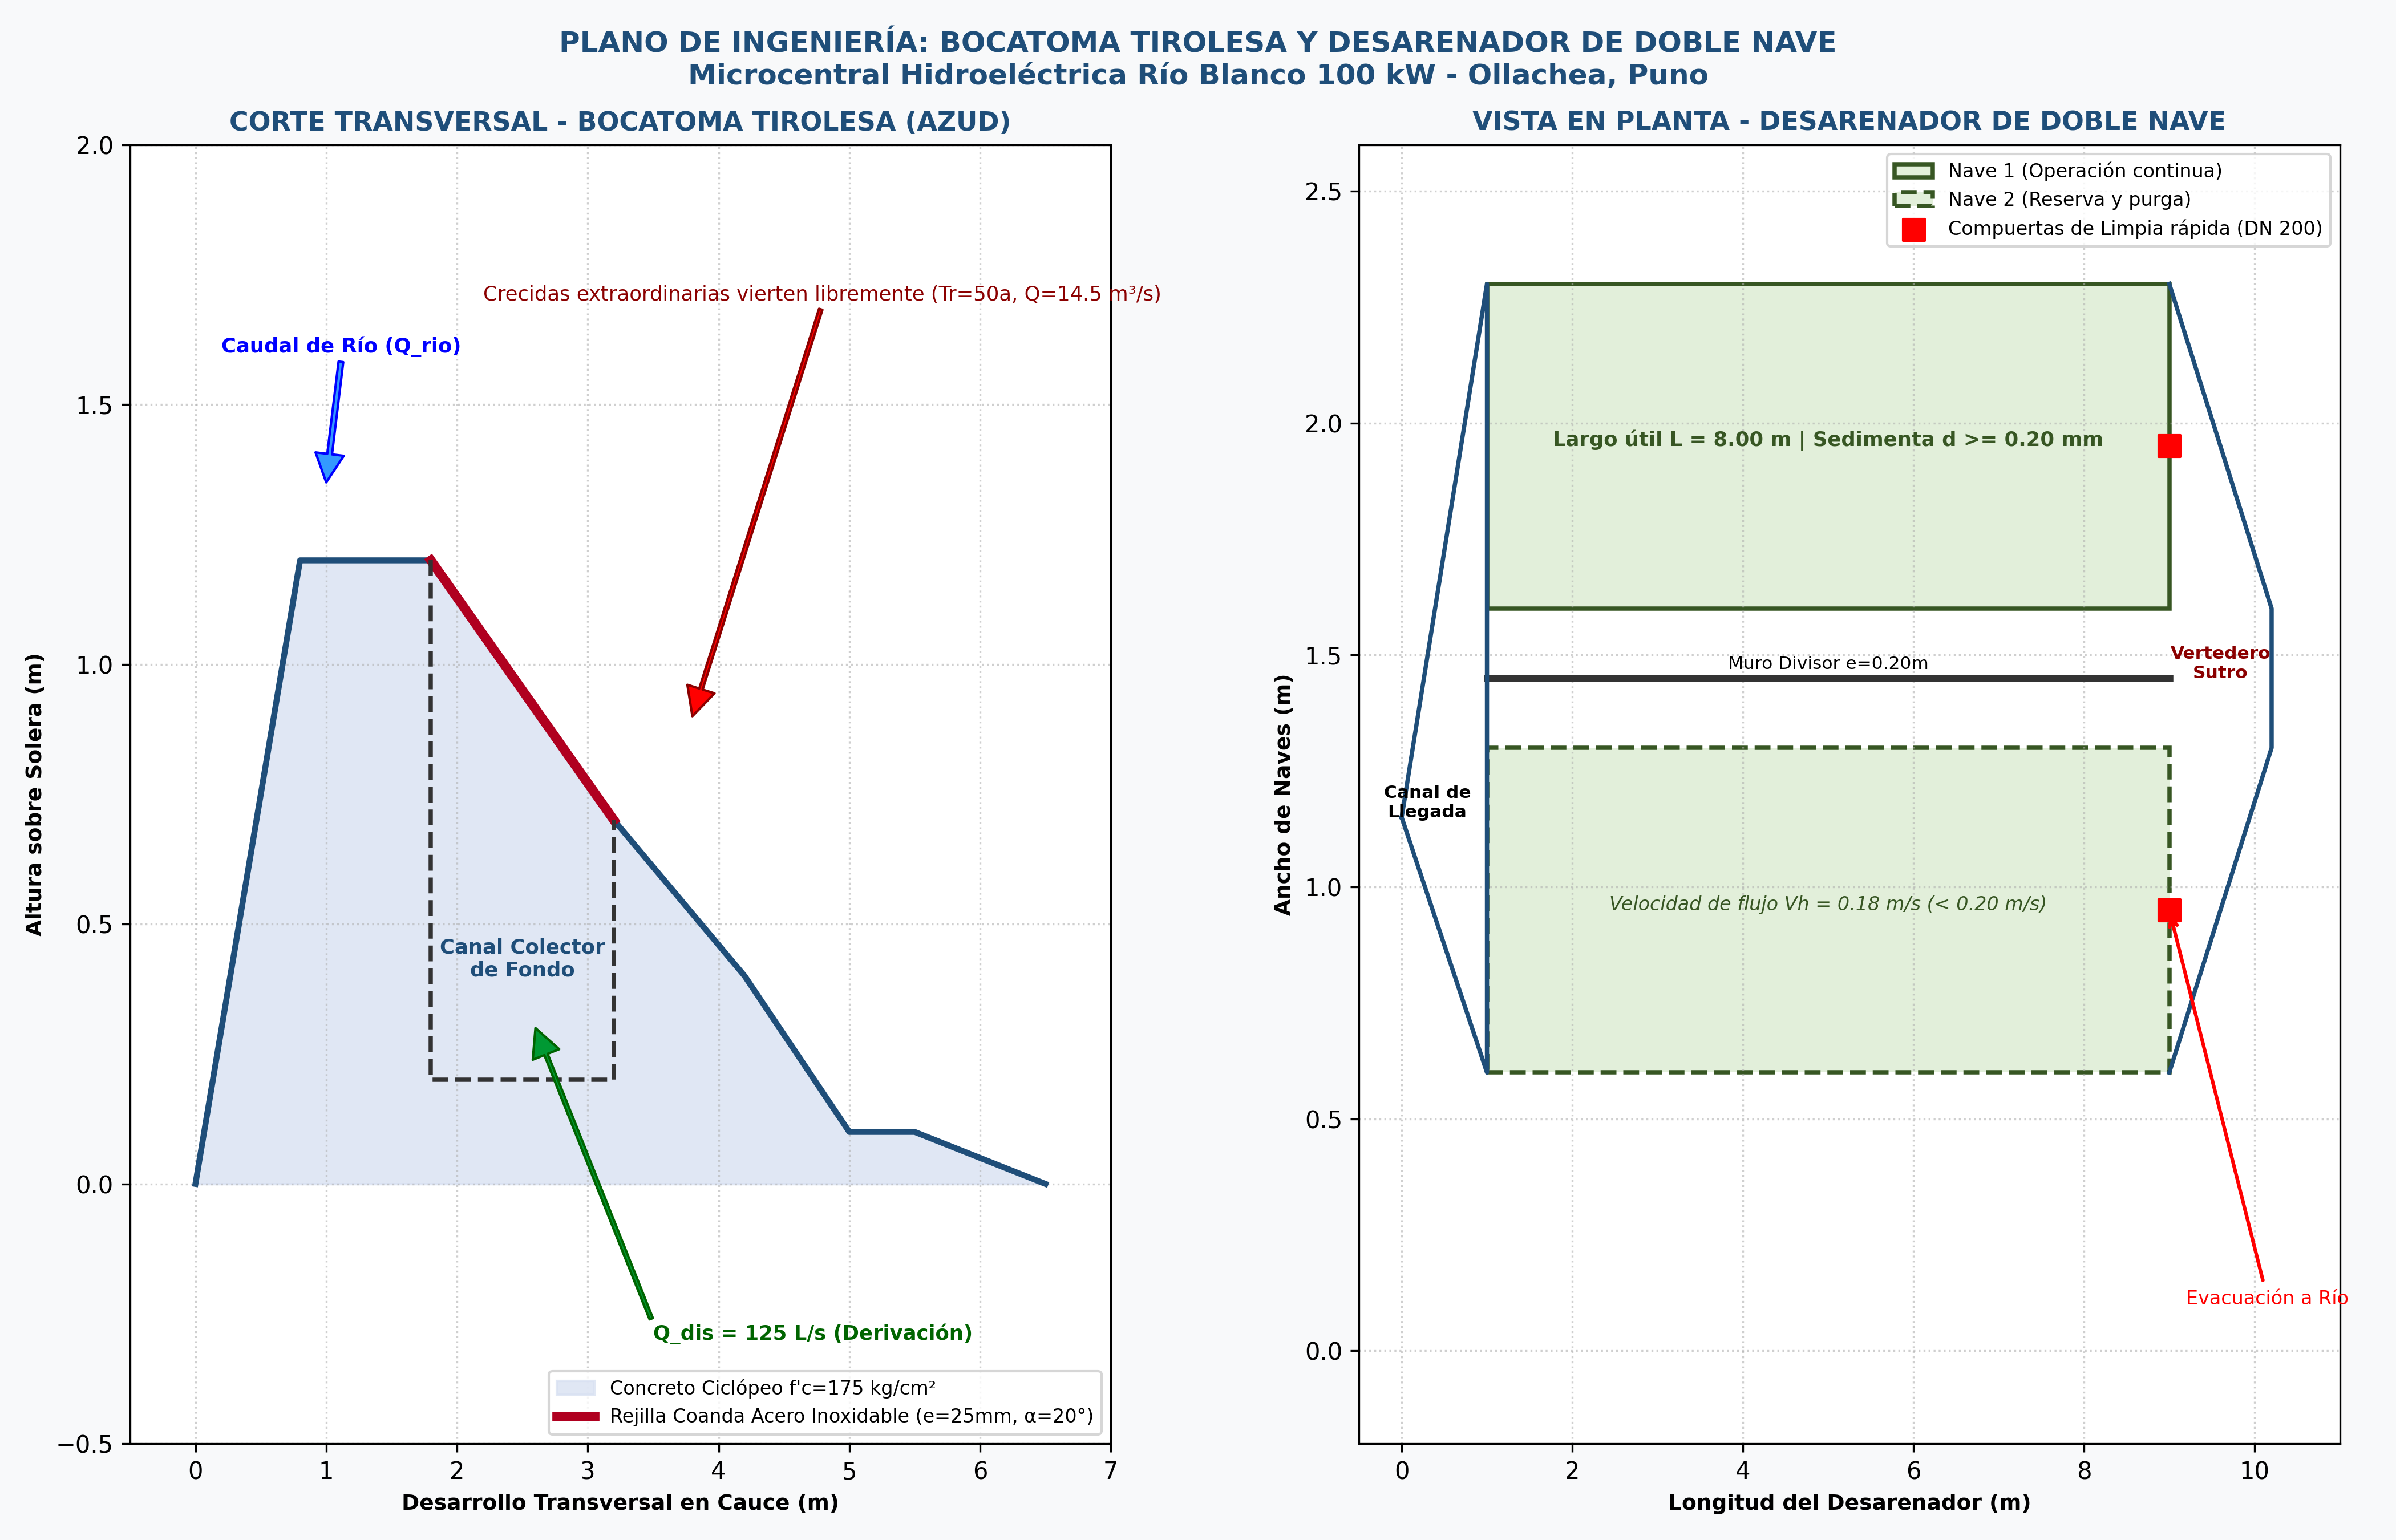
\includegraphics[width=0.92\linewidth]{../04 Mapas/Plano_01_Bocatoma_Tirolesa_Desarenador.png}
\caption{Plano de Detalle: Corte Transversal del Azud Tiroles y Vista en Planta del Desarenador de Doble Nave.}
\label{fig:plano1}
\end{figure}

\section{Desarenador de Doble Nave}
Para evitar el desgaste abrasivo de los inyectores y cucharas del rodete Pelton, se proyectó una cámara de sedimentación de doble nave dimensionada según la teoría de sedimentación de Camp y Hazzen para partículas de arena con diámetro $d \ge 0.20\text{ mm}$:
\begin{itemize}
    \item Velocidad de caída libre (Stokes): $w = 0.021\text{ m/s}$.
    \item Velocidad horizontal de flujo: $V_h = 0.18\text{ m/s}$ ($< 0.20\text{ m/s}$ para evitar resuspensión de sedimentos).
    \item Número de naves: 2 naves paralelas (permite limpieza de una nave sin paralizar la central).
    \item Dimensiones por nave: Longitud útil $L = 8.00\text{ m}$, ancho $b = 0.70\text{ m}$, profundidad $h = 1.10\text{ m}$.
    \item Vertedero de salida: Tipo proporcional Sutro para mantener velocidad constante.
    \item Sistema de purga: Válvulas de compuerta rápida DN 200 mm con descarga directa hacia el río.
\end{itemize}

\section{Canal de Aducción}
Canal rectangular abierto en concreto ciclópeo ($f'c = 175\text{ kg/cm}^2$) con longitud de $450\text{ m}$ a media ladera:
\begin{itemize}
    \item Ancho de solera: $b = 0.50\text{ m}$.
    \item Pendiente longitudinal: $S_0 = 0.0015$ ($1.5\text{ por mil}$).
    \item Coeficiente de rugosidad de Manning: $n = 0.014$.
    \item Tirante normal uniforme: $y_n = 0.331\text{ m}$.
    \item Bordo libre de seguridad: $F_b = 0.27\text{ m}$ (Altura total del canal $H = 0.60\text{ m}$).
    \item Velocidad media: $v = 0.755\text{ m/s}$.
    \item Número de Froude: $Fr = \frac{v}{\sqrt{g y_n}} = 0.419$ (Flujo subcrítico estable, libre de oleajes).
\end{itemize}

\section{Cámara de Carga (Forebay) y Aliviadero de Demasías}
Estructura de concreto armado de $4.00\text{ m} \times 3.00\text{ m} \times 2.20\text{ m}$ con capacidad útil de $22.5\text{ m}^3$ (equivalente a 3 minutos de turbinación nominal a plena carga), provista de rejilla fina limpiable con espaciamiento de 15 mm y compuerta plana de guarda.
La sumergencia hidráulica ($h_s$) para impedir la formación de vórtices y arrastre de aire a la tubería forzada se verificó mediante el criterio de Gordon:
\begin{equation}
h_{s,min} = 1.5 \cdot v \cdot \sqrt{D} = 1.5 \times 2.546 \times \sqrt{0.250} = 1.25\text{ m}
\end{equation}
Adoptándose una sumergencia efectiva de $h_s = 1.40\text{ m} > 1.25\text{ m}$ (CONFORME).

\begin{figure}[H]
\centering
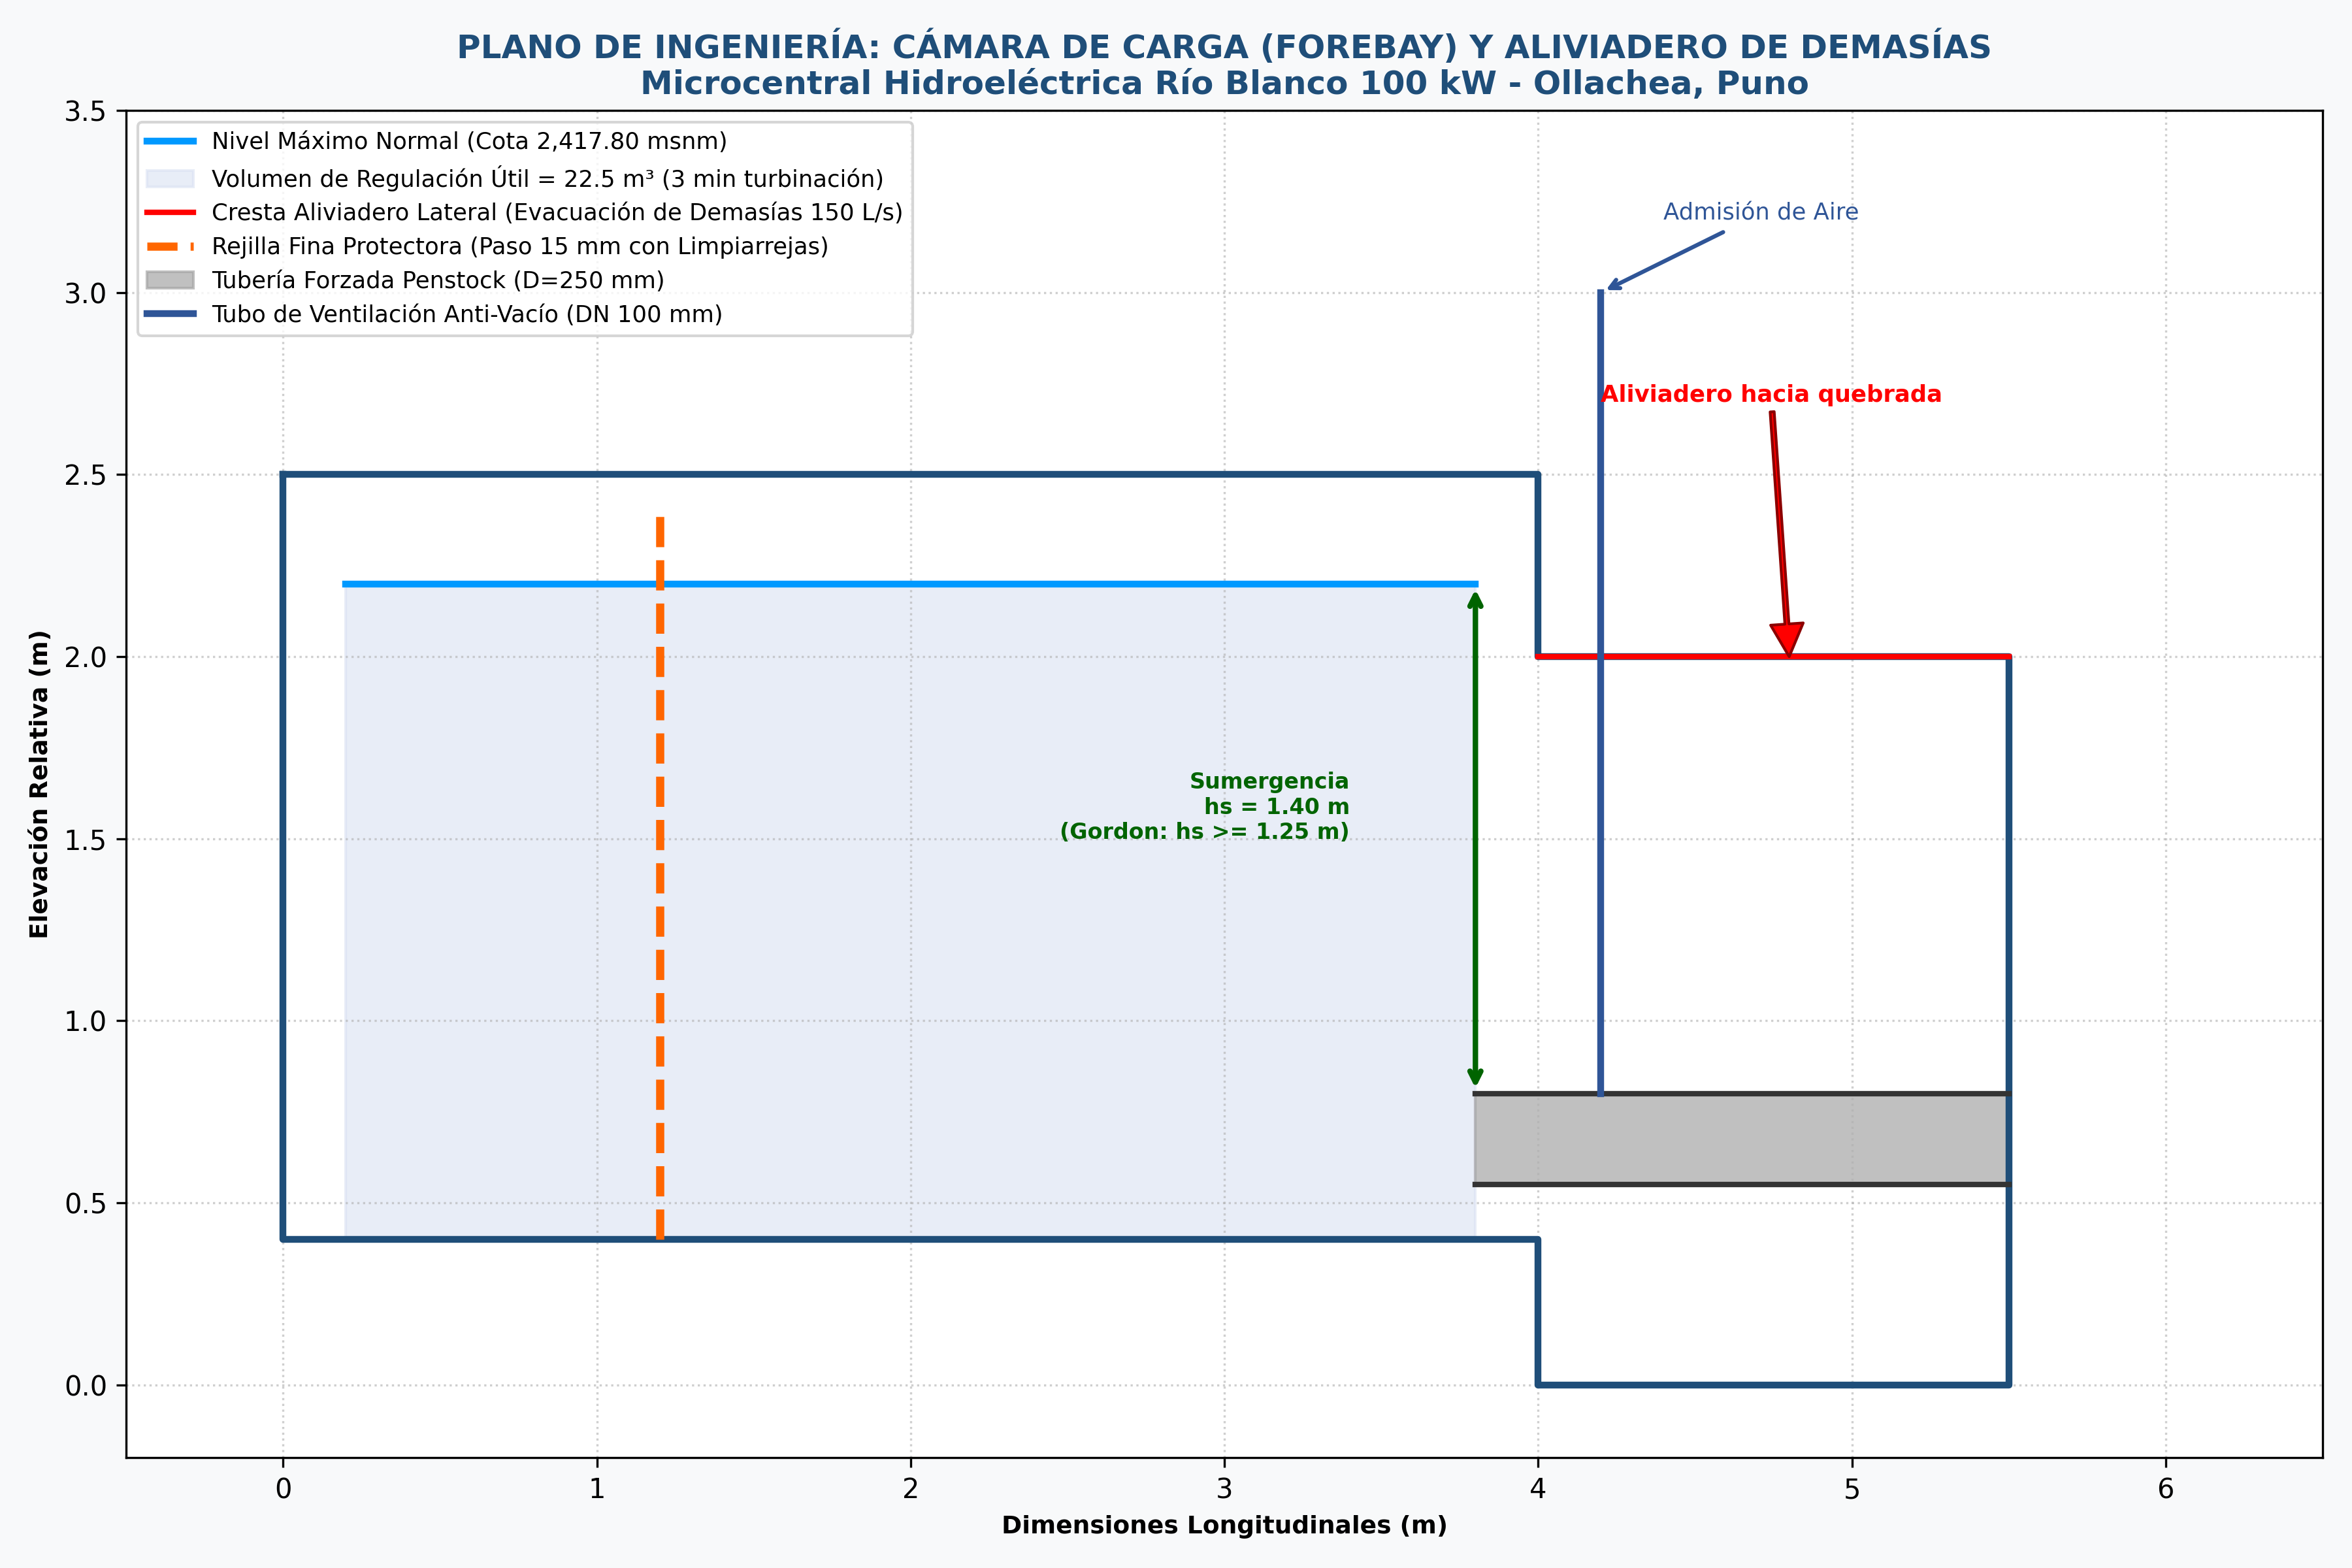
\includegraphics[width=0.92\linewidth]{../04 Mapas/Plano_02_Camara_Carga_Aliviadero.png}
\caption{Plano de Ingeniería: Cámara de Carga (Forebay), Aliviadero Lateral y Tubo Anti-Vacío.}
\label{fig:plano2}
\end{figure}

% CAPITULO 7
\chapter{Tubería Forzada, Transitorios Hidráulicos y Golpe de Ariete}
\section{Optimización del Diámetro Económico}
El diámetro de la tubería forzada se determinó aplicando las fórmulas empíricas consolidadas de Fahlbusch, Sarkaria y USBR:
\begin{equation}
D_{Fahlbusch} = 0.52 \cdot Q_d^{0.43} \cdot H_b^{0.14} = 0.52 \times (0.125)^{0.43} \times (115.0)^{0.14} = 0.246\text{ m}
\end{equation}
Adoptándose un diámetro interior nominal comercial de $D = 0.250\text{ m}$ (10 pulgadas), que garantiza una velocidad de flujo de $v_0 = 2.546\text{ m/s}$ (dentro del rango técnico-económico recomendado de 2.0 a 3.0 m/s).

\section{Pérdidas de Carga Hidráulica}
Para una longitud total desarrollada de $L = 380\text{ m}$ de tubería de acero ASTM A36 con rugosidad absoluta $k = 0.045\text{ mm}$ y número de Reynolds $Re = 517,577$, el factor de fricción de Darcy-Weisbach (Colebrook-White) es $f = 0.0153$.
\begin{equation}
h_f = f \cdot \frac{L}{D} \cdot \frac{v_0^2}{2g} = 0.0153 \times \frac{380}{0.250} \times \frac{2.546^2}{2 \times 9.81} = 7.67\text{ m}
\end{equation}
Las pérdidas localizadas singulares (embocadura abocinada, rejilla fina, 4 codos de radio amplio y válvula esférica de guarda) totalizan:
\begin{equation}
h_m = \sum K \frac{v_0^2}{2g} = 1.85 \times \frac{2.546^2}{2 \times 9.81} = 1.15\text{ m}
\end{equation}
\begin{equation}
h_{total} = h_f + h_m = 7.67 + 1.15 = 8.82\text{ m} \quad (7.67\% \text{ del salto bruto})
\end{equation}
\begin{equation}
H_n = H_b - h_{total} = 115.00 - 8.82 = 106.18\text{ m}
\end{equation}

\section{Transitorios Hidráulicos y Modelamiento de Golpe de Ariete}
La celeridad de la onda elástica de choque se calculó considerando la elasticidad del acero y la compresibilidad del agua:
\begin{equation}
a = \sqrt{\frac{K_{agua}}{\rho \left(1 + \frac{K_{agua}}{E_{acero}} \frac{D}{e}\right)}} = 1,195.79\text{ m/s}
\end{equation}
El tiempo de reflexión crítico de la onda es:
\begin{equation}
T_c = \frac{2 L}{a} = \frac{2 \times 380}{1,195.79} = 0.636\text{ s}
\end{equation}
Para evitar el embalamiento de la turbina Pelton ante un disparo fortuito de carga eléctrica, el sistema cuenta con deflectores mecánicos rápidos de chorro que actúan en $t_{def} = 0.50\text{ s}$, mientras que el servomotor de las toberas cierra gradualmente en un tiempo amortiguado de $t_c = 4.00\text{ s} > T_c$ (Régimen de Cierre Lento).
La sobrepresión según la ecuación de Allievi es:
\begin{equation}
\Delta H = \frac{2 L v_0}{g t_c} = \frac{2 \times 380 \times 2.546}{9.81 \times 4.00} = 49.32\text{ m.c.a.} \quad (42.9\% \text{ de } H_b)
\end{equation}
La presión máxima de diseño hidrodinámico alcanza:
\begin{equation}
P_{max} = H_b + \Delta H = 115.00 + 49.32 = 164.32\text{ m.c.a.} \quad (16.11\text{ bar})
\end{equation}

\begin{figure}[H]
\centering
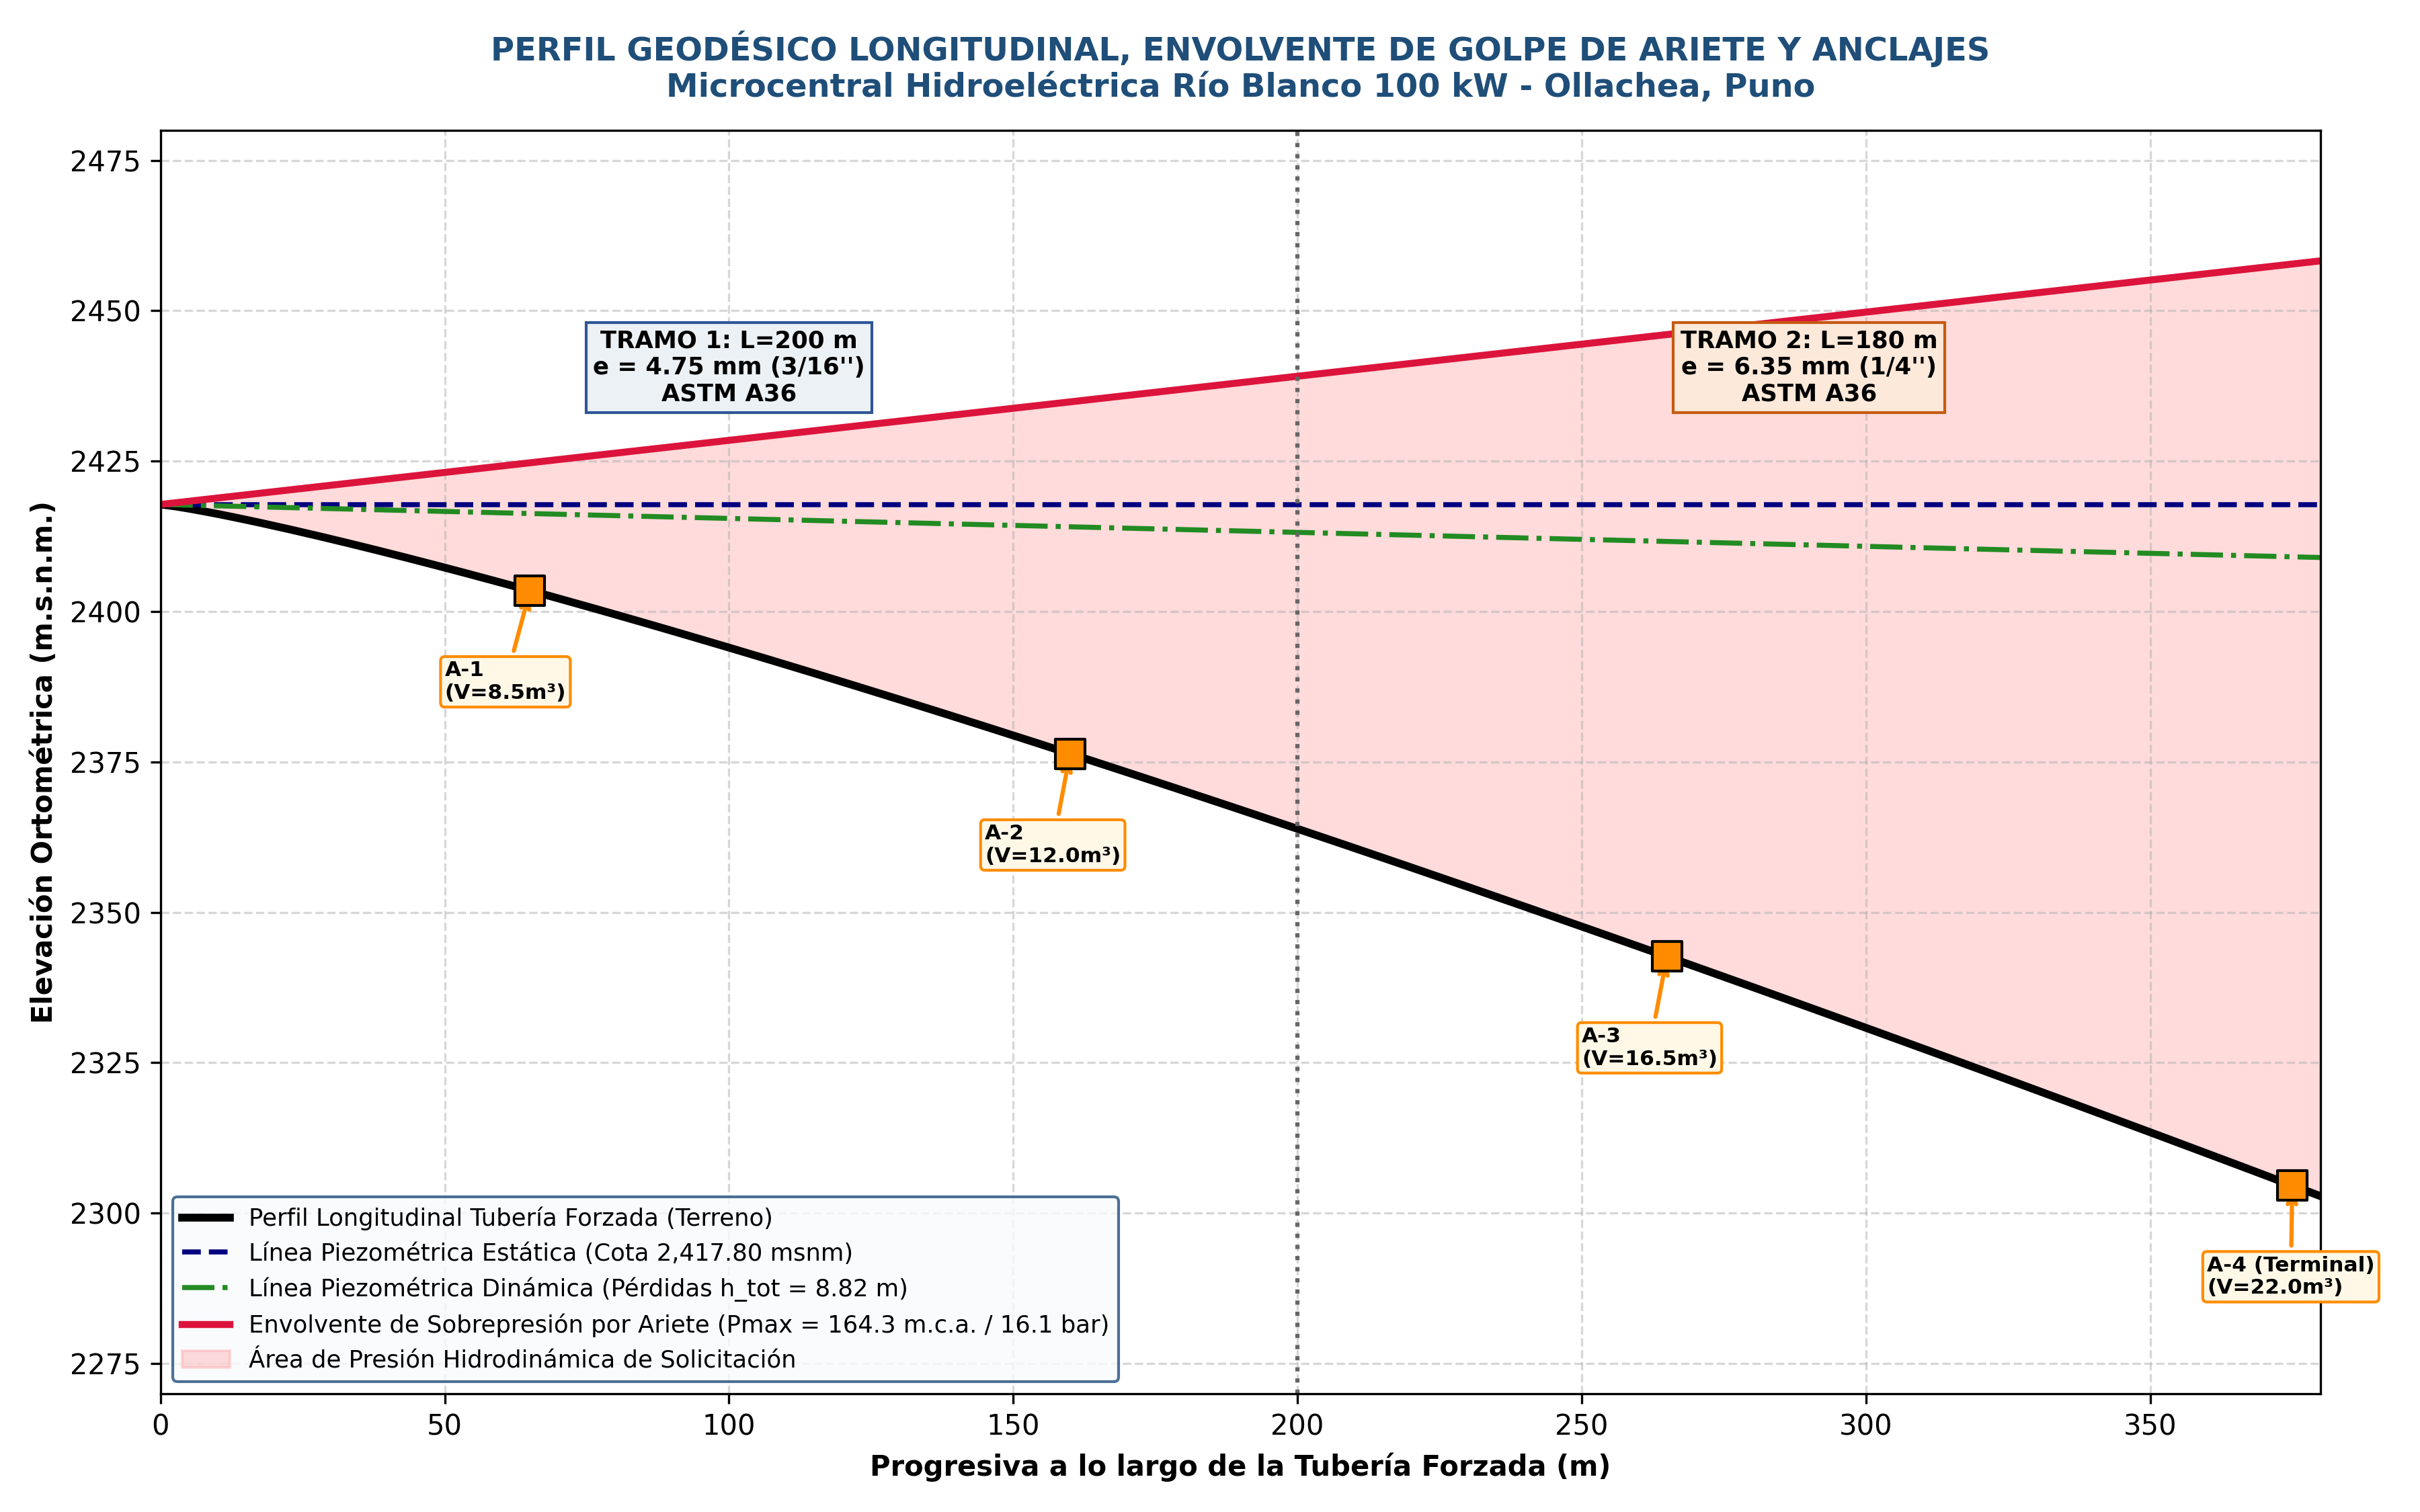
\includegraphics[width=0.92\linewidth]{../04 Mapas/Mapa_05_Perfil_Longitudinal_Tuberia_Forzada.png}
\caption{Perfil Geodésico Longitudinal, Envolvente de Golpe de Ariete y Ubicación de Bloques de Anclaje.}
\label{fig:mapa5}
\end{figure}

\section{Espesores de Tubería y Dados de Anclaje}
Aplicando la norma ASME B31.3 y AWWA M11 con un factor de seguridad $FS \ge 2.0$, eficiencia de junta $E_j = 0.85$ y sobre-espesor por corrosión de $1.5\text{ mm}$:
\begin{itemize}
    \item \textbf{Tramo Superior (0 a 200 m):} Espesor nominal adoptado: $4.75\text{ mm}$ (3/16 pulg) ($FS = 3.81$).
    \item \textbf{Tramo Inferior (200 a 380 m):} Espesor nominal adoptado: $6.35\text{ mm}$ (1/4 pulg) ($FS = 3.74$).
\end{itemize}

Para absorber los empujes hidrostáticos y las fuerzas dinámicas de cambio de cantidad de movimiento en los quiebres de ladera, se proponen conceptualmente cuatro bloques de anclaje de concreto ciclópeo ($f'c = 175\text{ kg/cm}^2 + 30\%$ PM):
\begin{itemize}
    \item \textbf{Anclaje A-1 (Prog. 0+065, Inflexión $18^\circ$):} Volumen de concreto: $8.5\text{ m}^3$.
    \item \textbf{Anclaje A-2 (Prog. 0+160, Inflexión $24^\circ$):} Volumen de concreto: $12.0\text{ m}^3$.
    \item \textbf{Anclaje A-3 (Prog. 0+265, Inflexión $31^\circ$):} Volumen de concreto: $16.5\text{ m}^3$.
    \item \textbf{Anclaje A-4 Terminal (Prog. 0+375, Inflexión $15^\circ$):} Volumen de concreto: $22.0\text{ m}^3$.
\end{itemize}

% CAPITULO 8
\chapter{Diseño Electromecánico: Turbina Pelton y Generador Síncrono}
\section{Selección y Dimensionamiento del Rodete Pelton}
Para un salto neto de $H_n = 106.18\text{ m}$ y caudal de $Q_d = 125\text{ L/s}$, la velocidad específica $n_s = 18.5\text{ rpm}\cdot(\text{kW})^{0.5}/\text{m}^{1.25}$ ubica al proyecto en la zona de máximo rendimiento de una turbina de acción Pelton de 2 inyectores.

\begin{figure}[H]
\centering
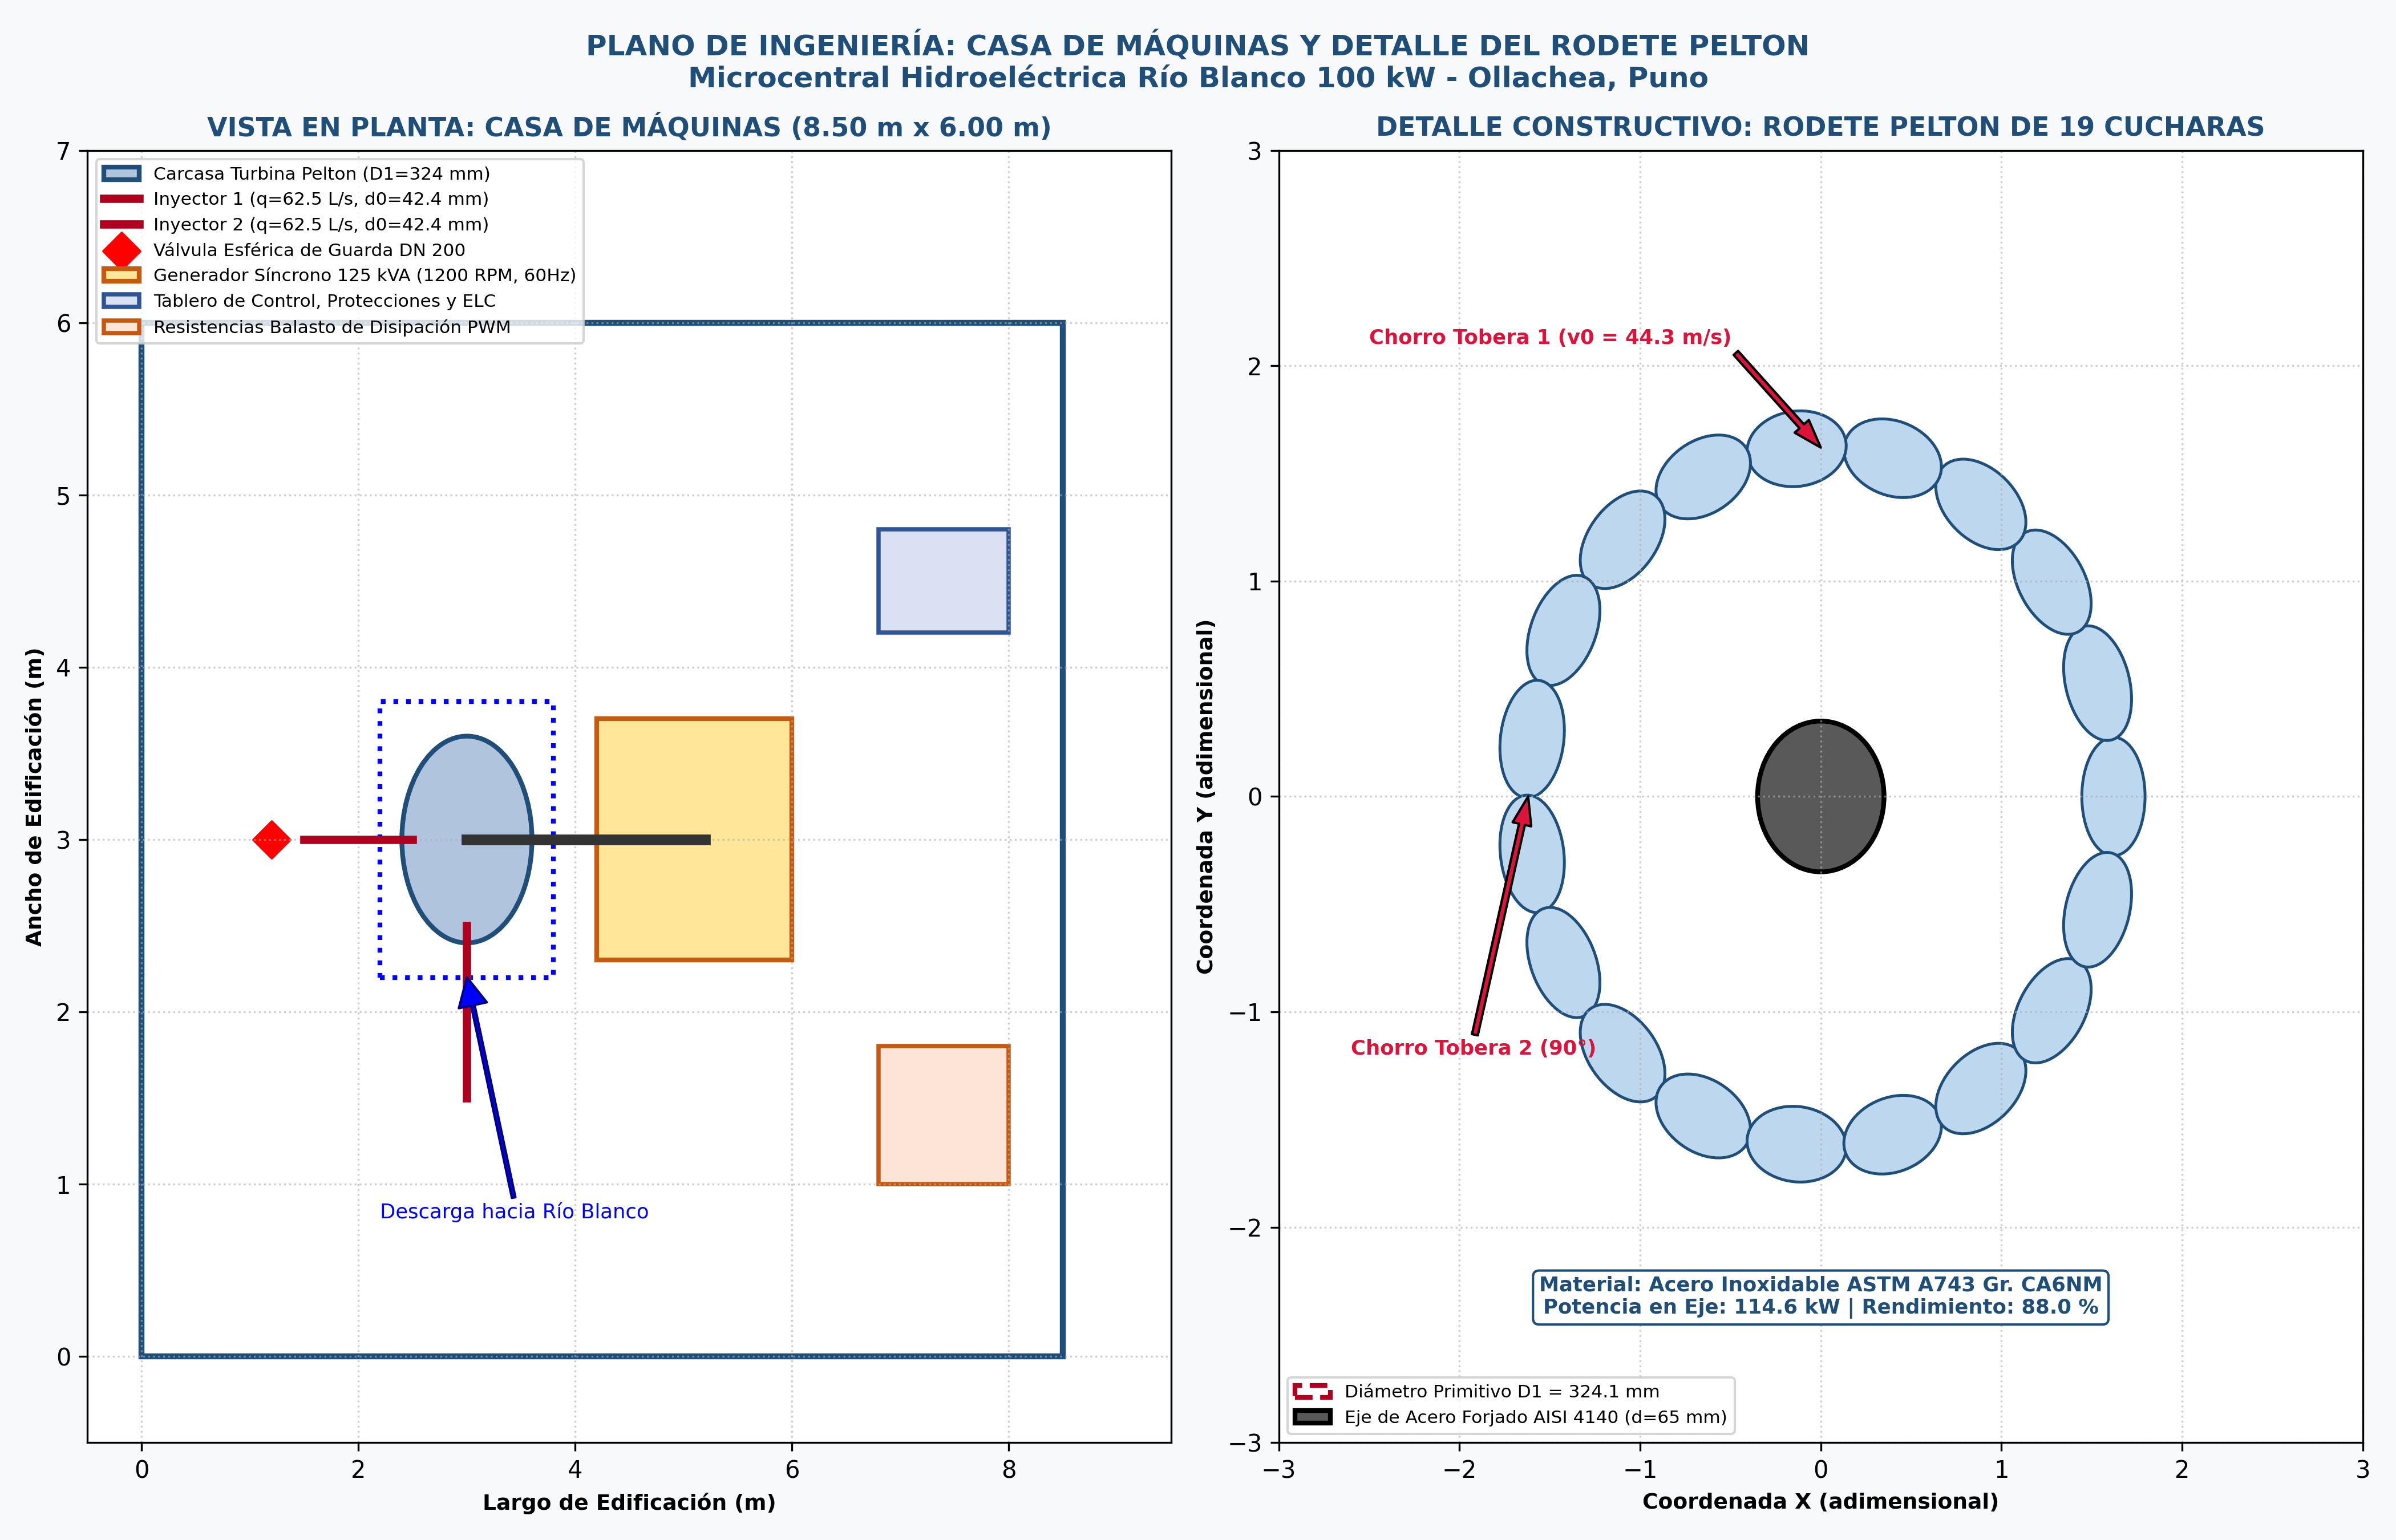
\includegraphics[width=0.92\linewidth]{../04 Mapas/Plano_03_Casa_Maquinas_Grupo_Pelton.png}
\caption{Plano de Ingeniería: Disposición de Casa de Máquinas y Geometría del Rodete Pelton de 19 Cucharas.}
\label{fig:plano3}
\end{figure}

\begin{table}[H]
\centering
\small
\begin{tabularx}{\linewidth}{lX}
\toprule
\textbf{Parámetro Técnico} & \textbf{Valor de Diseño / Especificación} \\
\midrule
Tipo de Turbina & Pelton de eje horizontal monobloque con 2 inyectores \\
Caudal Nominal Turbinado ($Q_d$) & $0.125\text{ m}^3/\text{s}$ ($125.0\text{ L/s}$ total, $62.5\text{ L/s}$ por tobera) \\
Salto Hidráulico Neto ($H_n$) & $106.18\text{ m}$ \\
Velocidad del Chorro ($v_0$) & $44.27\text{ m/s}$ (Coeficiente de tobera $C_v = 0.97$) \\
Diámetro de Tobera / Chorro ($d_0$) & $42.4\text{ mm}$ \\
Velocidad Sincrónica de Giro ($N$) & $1,200\text{ RPM}$ (Directo al alternador de 6 polos a 60 Hz) \\
Velocidad de Embalamiento ($N_r$) & $2,184\text{ RPM}$ ($1.82 \times N_{nom}$) \\
Diámetro Primitivo del Rodete ($D_1$) & $324.1\text{ mm}$ (Relación $D_1/d_0 = 7.65$) \\
Número de Cucharas ($Z$) & 19 cucharas monobloque (Fórmula de Taygun / Nechleba) \\
Dimensiones de Cucharas & Ancho $B = 127.2\text{ mm}$, Largo $L = 110.2\text{ mm}$, Prof. $T = 42.4\text{ mm}$ \\
Material del Rodete & Acero Inoxidable ASTM A743 Grado CA6NM (13\% Cr, 4\% Ni) \\
Rendimiento de la Turbina ($\eta_t$) & $88.0\%$ \\
Potencia Mecánica en el Eje ($P_{mec}$) & $114.58\text{ kW}$ (Momento torsor nominal $T = 911.8\text{ N}\cdot\text{m}$) \\
Eje de Transmisión & Acero aleado forjado AISI 4140, diámetro $d = 65\text{ mm}$ \\
\bottomrule
\end{tabularx}
\caption{Ficha Técnica de Diseño del Grupo Turbina Pelton Río Blanco.}
\label{tab:pelton}
\end{table}

\section{Generador Eléctrico Síncrono}
\begin{itemize}
    \item \textbf{Tipo:} Generador síncrono trifásico autoexcitado sin escobillas (Brushless).
    \item \textbf{Potencia Aparente Nominal:} $125.0\text{ kVA}$.
    \item \textbf{Potencia Activa Nominal:} $106.25\text{ kW}$ ($\cos\phi = 0.85$ inductivo).
    \item \textbf{Tensión Nominal / Frecuencia:} $400 / 230\text{ V}$ trifásico, 4 hilos, $60\text{ Hz}$.
    \item \textbf{Corriente Nominal:} $180.4\text{ A}$.
    \item \textbf{Velocidad / Polos:} $1,200\text{ RPM}$ (6 polos).
    \item \textbf{Rendimiento a Plena Carga:} $93.0\%$.
    \item \textbf{Sistema de Excitación:} PMG con regulador automático de voltaje (AVR) digital ($\pm 0.5\%$).
    \item \textbf{Aislamiento / Protección:} Clase H con elevación de temperatura Clase F, protección IP54.
\end{itemize}

\section{Regulador Electrónico de Carga (ELC)}
El control de velocidad y frecuencia ($60.0 \pm 0.2\text{ Hz}$) se confía a un Regulador Electrónico de Carga (ELC) trifásico modulado por ancho de pulsos (PWM) con transistores IGBT. El ELC desvía instantáneamente la potencia no consumida hacia un banco resistivo balasto de $120\text{ kW}$ sumergido en un tanque de agua secundaria acoplado al canal de descarga, garantizando cero perturbaciones de frecuencia ante desconexiones intempestivas de cargas rurales.

% CAPITULO 9
\chapter{Sistema Eléctrico, Subestación 0.38/10 kV y Conexión a Red}
\section{Esquema Unifilar y Protecciones Eléctricas}
El sistema eléctrico centraliza las funciones de generación, compensación reactiva, seccionamiento y elevación de tensión hacia la red rural.

\begin{figure}[H]
\centering
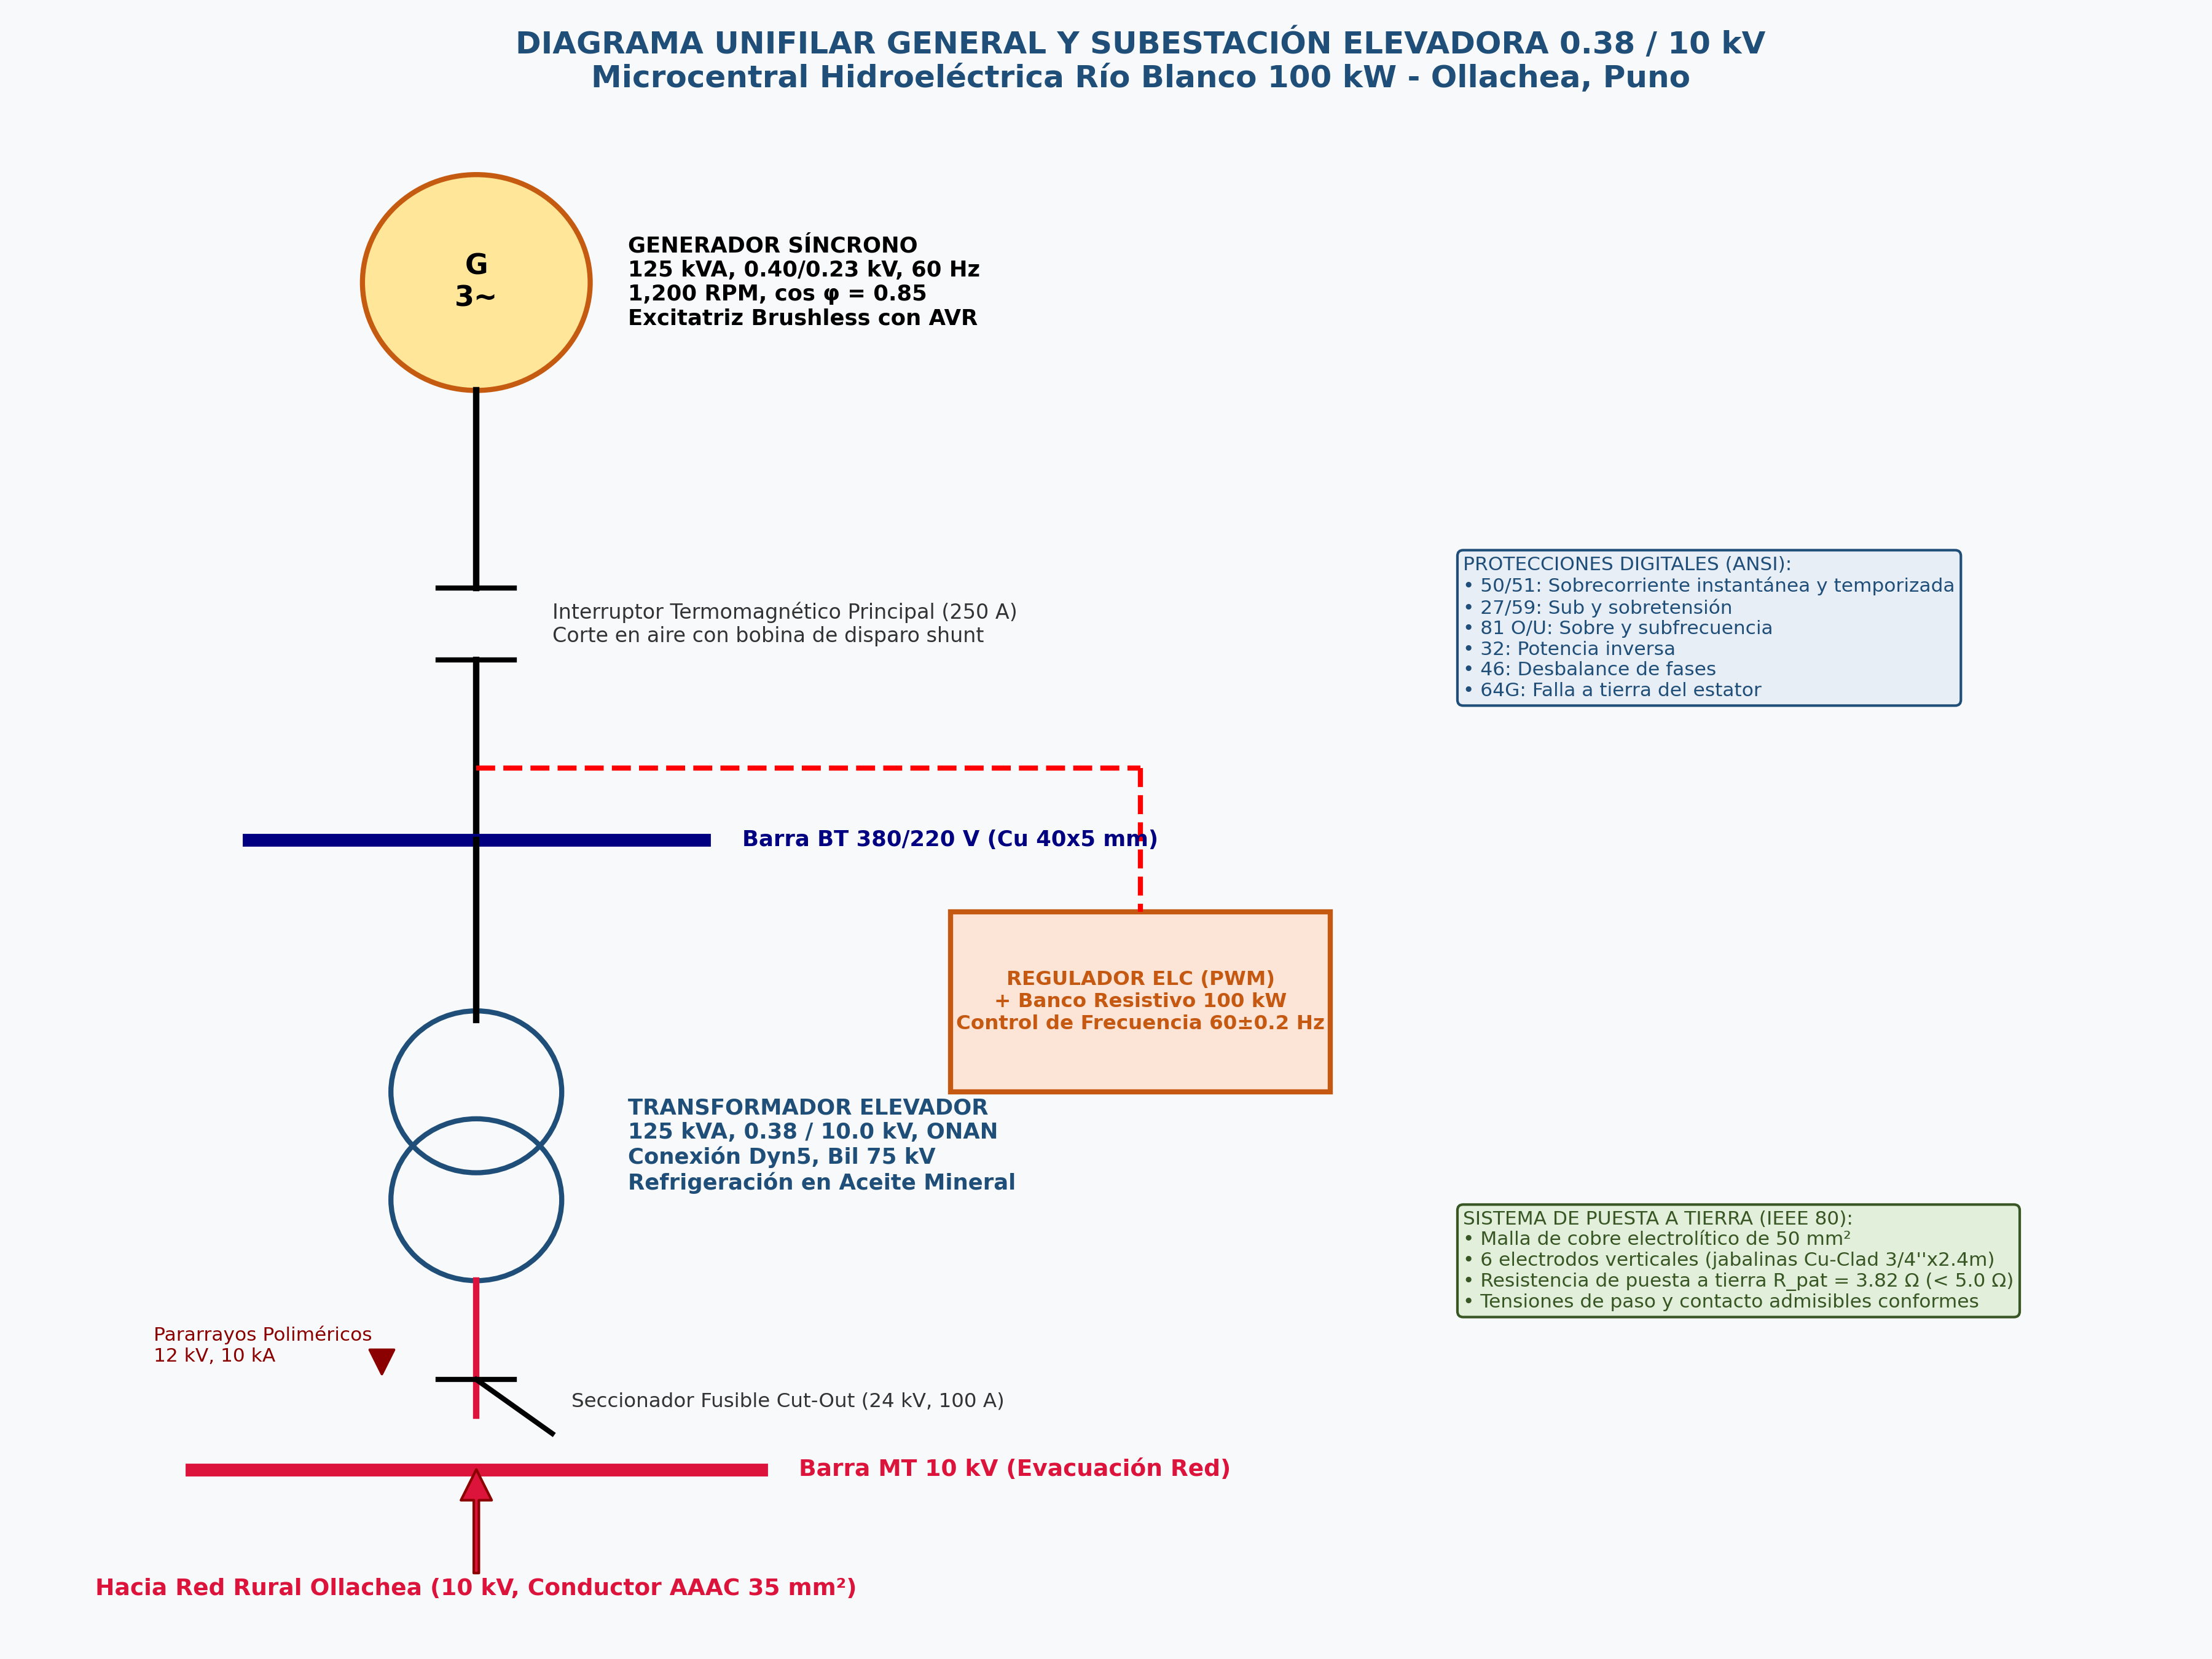
\includegraphics[width=0.92\linewidth]{../04 Mapas/Plano_04_Diagrama_Unifilar_Subestacion.png}
\caption{Diagrama Unifilar General, Subestación Elevadora 0.38/10 kV y Malla de Puesta a Tierra.}
\label{fig:plano4}
\end{figure}

El relé multifunción digital integra las siguientes protecciones ANSI:
\begin{itemize}
    \item \textbf{ANSI 50/51:} Sobrecorriente instantánea y temporizada de fase y neutro.
    \item \textbf{ANSI 27/59:} Subtensión ($0.85 U_n$) y sobretensión ($1.15 U_n$).
    \item \textbf{ANSI 81 O/U:} Sobrefrecuencia ($62.0\text{ Hz}$) y subfrecuencia ($57.5\text{ Hz}$).
    \item \textbf{ANSI 32:} Potencia inversa (evita que el alternador opere como motor sincrónico).
    \item \textbf{ANSI 46:} Desbalance de fases y corriente de secuencia negativa.
    \item \textbf{ANSI 64G:} Protección contra falla a tierra en estator.
\end{itemize}

\section{Subestación Elevadora y Línea de Media Tensión}
\begin{itemize}
    \item \textbf{Transformador de Potencia:} $125\text{ kVA}$, trifásico, baño de aceite mineral ONAN, relación $0.380 / 10.0\text{ kV}$, grupo de conexión Dyn5 con neutro sólidamente aterrado, $u_k = 4.5\%$.
    \item \textbf{Línea de Media Tensión (10 kV):} Longitud de $3.2\text{ km}$ sobre postes de concreto armado centrifugado de 12 m, conductor de aleación de aluminio AAAC de $35\text{ mm}^2$. La caída de tensión calculada es de apenas $0.41\%$ ($41.2\text{ V}$), inferior al límite reglamentario del $5\%$.
\end{itemize}

\section{Sistema de Puesta a Tierra (IEEE Std 80)}
Malla de tierra profunda de $8.0\text{ m} \times 6.0\text{ m}$ construida con cable de cobre electrolítico desnudo de $50\text{ mm}^2$ enterrado a $0.60\text{ m}$, equipada con 8 jabalinas Copperweld de $3/4'' \times 2.40\text{ m}$ tratadas con bentonita sódica. La resistencia resultante es de $R_{pat} = 3.79\,\Omega$, cumpliendo con el CNE ($R_{pat} \le 5.0\,\Omega$).

% CAPITULO 10
\chapter{Aplicaciones y Usos Productivos de la Energía Eléctrica}
\section{Diagnóstico de la Demanda y Zonificación Energética}
El dimensionamiento de la microcentral trasciende la simple cobertura lumínica domiciliaria, articulando un plan maestro de electrificación y desarrollo agroindustrial sostenible para las comunidades del entorno de Ollachea.

\begin{figure}[H]
\centering
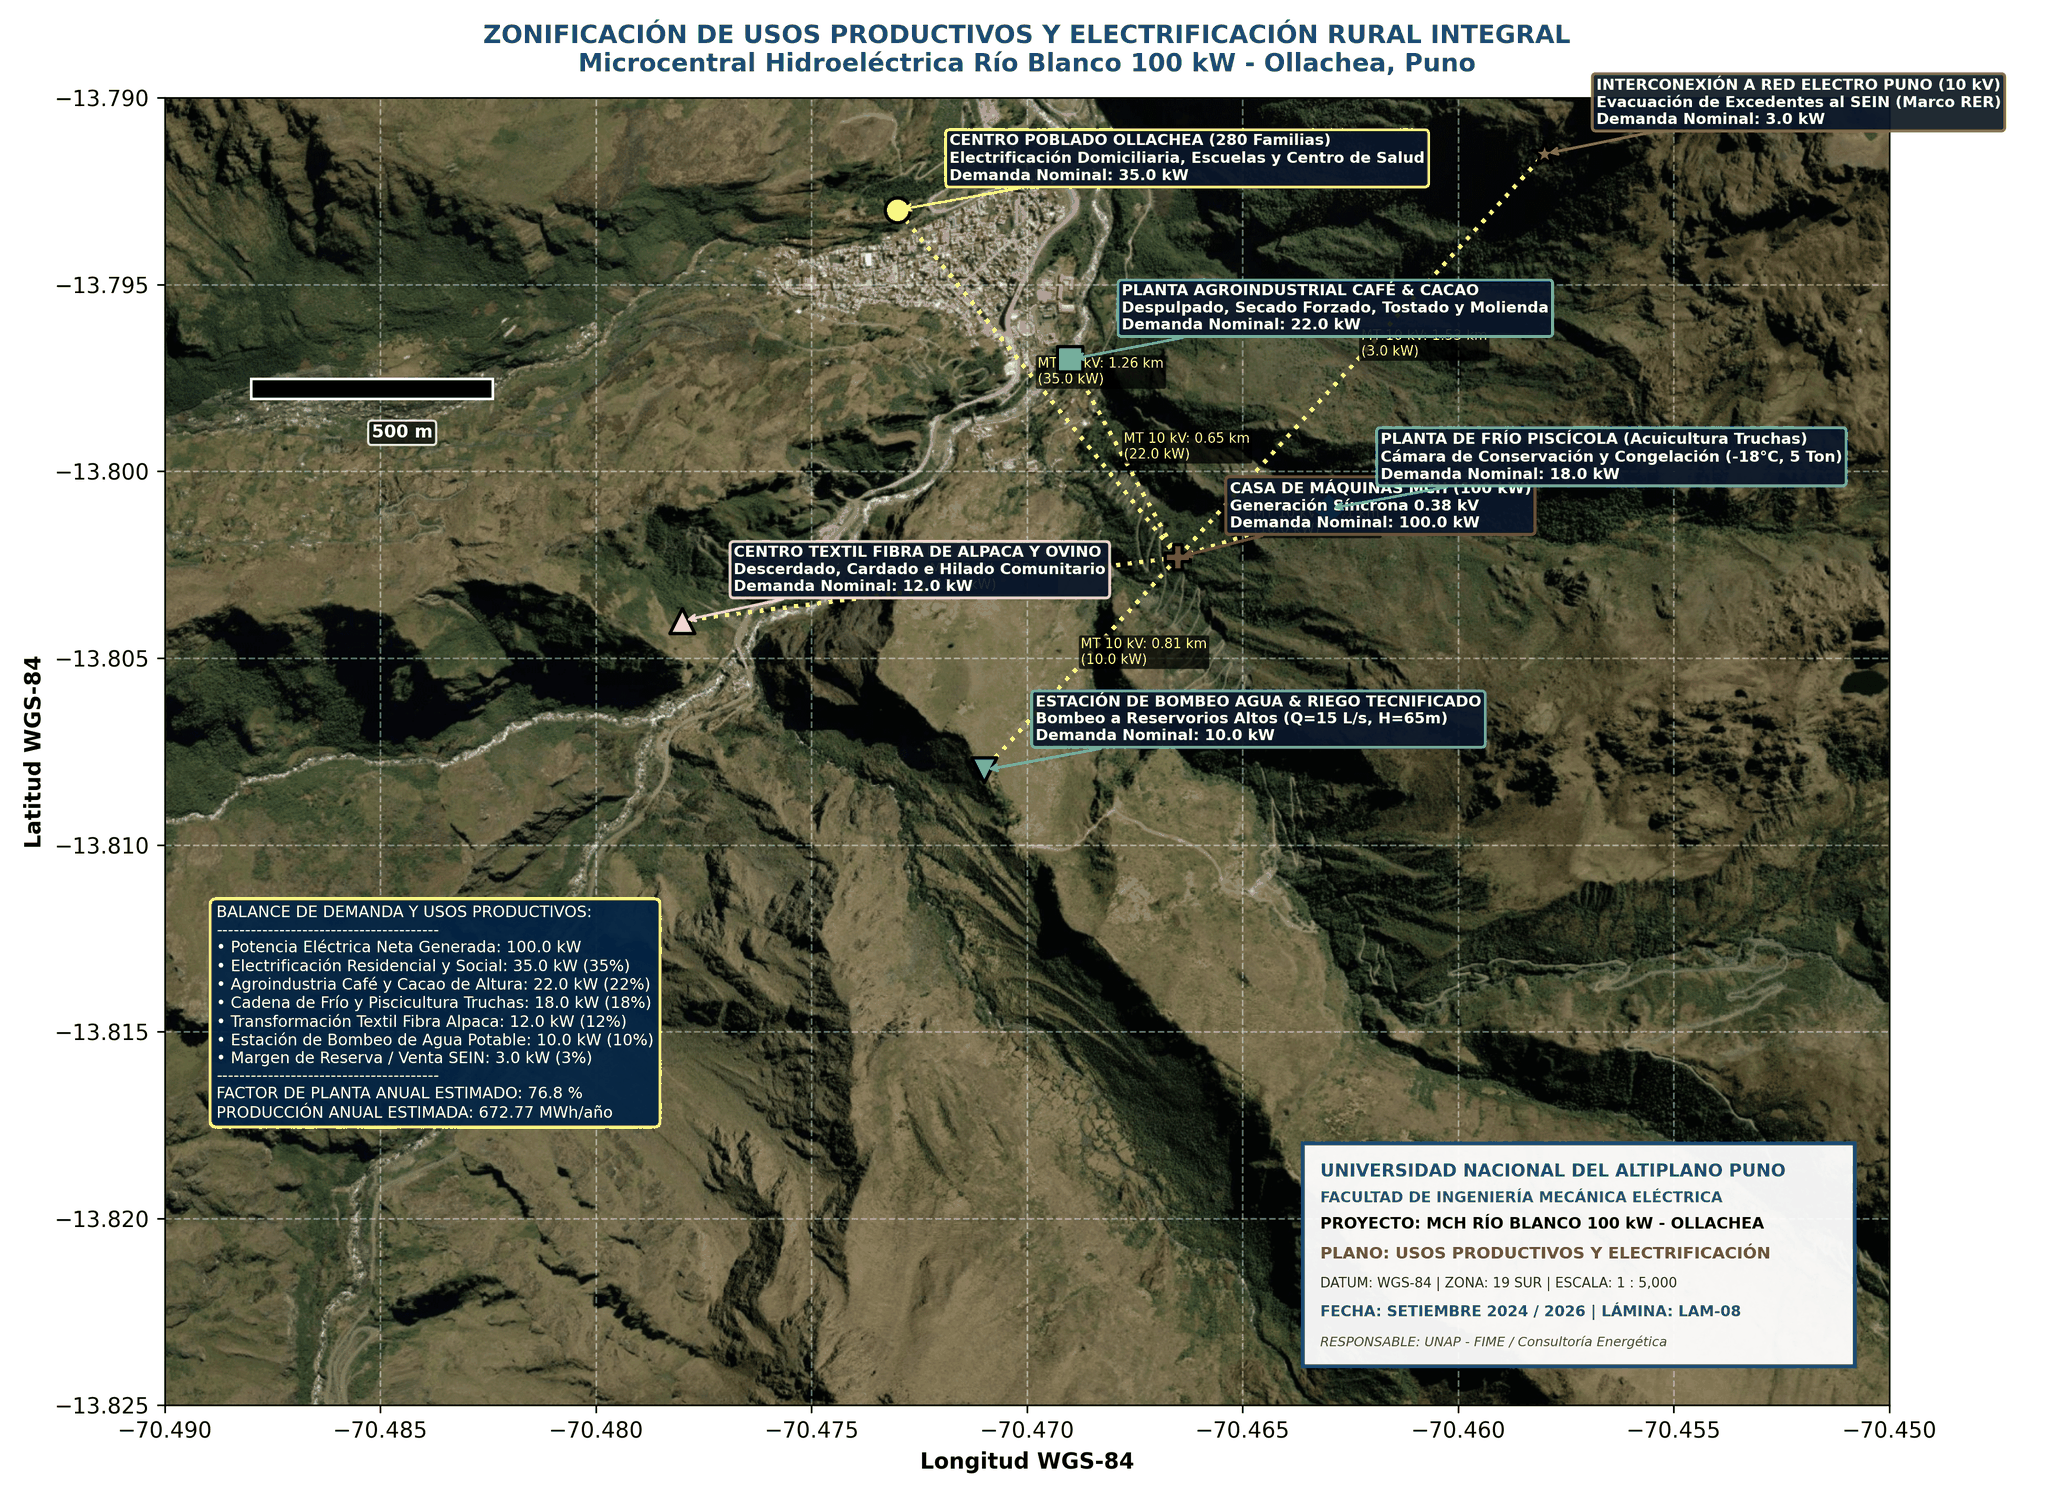
\includegraphics[width=0.92\linewidth]{../04 Mapas/Mapa_08_Zonificacion_Usos_Productivos_Electrificacion.png}
\caption{Mapa de Zonificación de Usos Productivos, Centros de Carga y Red Eléctrica Rural.}
\label{fig:mapa8}
\end{figure}

\begin{table}[H]
\centering
\small
\begin{tabularx}{\linewidth}{lXcc}
\toprule
\textbf{Centro de Carga / Aplicación} & \textbf{Descripción del Proceso y Equipamiento} & \textbf{Potencia [kW]} & \textbf{Proporción (\%)} \\
\midrule
Electrificación Domiciliaria y Social & 280 familias campesinas, alumbrado público LED, 2 colegios con aulas de cómputo y posta de salud & 35.0 kW & 35.0\% \\
Planta Agroindustrial Café y Cacao & Despulpado mecánico, secado por convección forzada con aire caliente limpio, tostadora y molienda & 22.0 kW & 22.0\% \\
Cadena de Frío para Piscicultura & Cámara frigorífica comunitaria de conservación y congelación ($-18^\circ\text{C}$, 5 Ton) y sopladores de aireación & 18.0 kW & 18.0\% \\
Transformación de Fibra de Alpaca & Centro de acopio comunal con descerdadoras, cardadoras e hiladoras textiles eléctricas & 12.0 kW & 12.0\% \\
Bombeo de Agua Potable y Riego & Electrobombas sumergibles para elevación de agua potable a reservorios y riego tecnificado & 10.0 kW & 10.0\% \\
Reserva Operativa y Venta SEIN & Margen de regulación dinámica e inyección de excedentes a la red de Electro Puno S.A.A. & 3.0 kW & 3.0\% \\
\midrule
\textbf{Total Potencia Neta Demandada} & \textbf{Balance Integral de Generación y Cargas Comunitarias} & \textbf{100.0 kW} & \textbf{100.0\%} \\
\bottomrule
\end{tabularx}
\caption{Distribución y Balance de Cargas para Usos Productivos en Ollachea.}
\label{tab:usos_productivos}
\end{table}

\section{Detalle de las Principales Cadenas Productivas Beneficiadas}
\subsection{Agroindustria de Café de Altura y Cacao (Carabaya)}
Los valles de Ollachea y San Gabán producen café arábica de alta especialidad que tradicionalmente perdía valor comercial por el secado artesanal a la intemperie en épocas lluviosas. La microcentral proveerá energía limpia para:
\begin{itemize}
    \item Dos despulpadoras mecánicas de bajo consumo hídrico ($2 \times 3.0\text{ kW}$).
    \item Cuatro secadores mecánicos de tambor rotatorio con ventilación forzada ($4 \times 2.5\text{ kW}$).
    \item Una tosta-enfriadora y dos molinos de muelas de precisión ($6.0\text{ kW}$).
\end{itemize}

\subsection{Cadena de Frío para Acuicultura de Truchas}
La crianza de trucha arcoíris (\textit{Oncorhynchus mykiss}) en el Río Blanco requiere mantener la cadena de frío para evitar la descomposición del producto eviscerado con destino al mercado regional de Juliaca y Cusco:
\begin{itemize}
    \item Cámara de congelación rápida de 5 toneladas métricas con compresor semi-hermético de $12.0\text{ kW}$.
    \item Fabricadora de hielo en escamas de $2\text{ Ton/día}$ ($4.0\text{ kW}$).
    \item Dos sopladores tipo Roots para oxigenación forzada en piscinas de alevines ($2 \times 1.0\text{ kW}$).
\end{itemize}

\subsection{Procesamiento de Fibra de Camélidos Sudamericanos (Alpaca Huacaya y Suri)}
La instalación de un módulo electromecánico de descerdado mecánico incrementa el valor de la fibra de alpaca de USD 3.50/lb (fibra en broza) a más de USD 18.00/lb (tops e hilado limpio), beneficiando de forma directa a los criadores comuneros de las zonas altas de Carabaya.

% CAPITULO 11
\chapter{Evaluación de Impacto Ambiental, Social y Plan de Manejo (PMA)}
\section{Categorización Ambiental (SENACE / MINEM)}
De acuerdo con el Reglamento de Protección Ambiental para las Actividades Eléctricas (D.S. N$^\circ$ 014-2019-EM) y el marco del SEIA (Ley N$^\circ$ 27446), la MCH Río Blanco clasifica como proyecto con impactos ambientales negativos leves, correspondiéndole el instrumento de Declaración de Impacto Ambiental (DIA). Al ser una central hidroeléctrica de pasada (run-of-river):
\begin{itemize}
    \item No existe embalse ni inundación de valles agrícolas o pastizales.
    \item No se produce alteración del régimen limnológico de caudales aguas abajo del punto de restitución.
    \item No se generan emisiones de gases de efecto invernadero (GEI), evitando la emisión de aproximadamente $450\text{ toneladas de CO}_2\text{ eq/año}$ frente a generación con diésel.
\end{itemize}

\section{Plan de Manejo Ambiental (PMA)}
\begin{itemize}
    \item \textbf{Control del Caudal Ecológico:} Monitoreo telemétrico continuo y vertedero calibrado fijo que garantiza en todo momento el flujo ininterrumpido de $30\text{ L/s}$ en el cauce natural.
    \item \textbf{Prevención de Erosión y Revegetación:} Estabilización biológica de las bermas del canal y zanja del penstock mediante la siembra de queñua (\textit{Polylepis racemosa}), colle y pastos andinos nativos.
    \item \textbf{Manejo de Residuos Sólidos y Sustancias Peligrosas:} Uso exclusivo de aceites y grasas lubricantes biodegradables en chumaceras y compuertas; los escombros de excavación ($1,250\text{ m}^3$) serán dispuestos en el Depósito de Material Excedente (DME) comunal autorizado.
\end{itemize}

% CAPITULO 12
\chapter{Plan de Operación, Mantenimiento y Gestión del Riesgo de Desastres}
\section{Estrategia de Mantenimiento Preventivo y Predictivo}
Para garantizar una disponibilidad operativa superior al $96.5\%$ durante los 30 años de vida útil de la central:
\begin{itemize}
    \item \textbf{Régimen Diario / Semanal:} Limpieza manual de hojas y ramas en rejilla tirolesa y cámara de carga; purga de sedimentos finos en el desarenador de doble nave; verificación de presión hidrostática y lubricación de cojinetes.
    \item \textbf{Régimen Mensual:} Inspección visual del trazo del canal y juntas Dresser en tubería forzada; prueba de disparo simulado del relé multifunción de protecciones ANSI; limpieza de filtros del sistema de excitación y ELC.
    \item \textbf{Régimen Anual (Parada Programada de 3 días en estiaje):} Inspección con líquidos penetrantes en las raíces de las 19 cucharas del rodete Pelton para descartar microfisuras por fatiga; recalibración de agujas e inyectores; reposición de pintura epóxica alquitrán en el interior del penstock; medición de la resistencia de la malla a tierra.
\end{itemize}

\section{Plan de Gestión del Riesgo de Desastres (PGRD)}
\begin{itemize}
    \item \textbf{Riesgo de Avenidas Extraordinarias:} El vertedero del azud cuenta con capacidad para evacuar hasta $3.56\text{ m}^3/\text{s}$ (Tr=50a) y $3.77\text{ m}^3/\text{s}$ (Tr=100a) con un bordo libre remanente de 0.85 m en los estribos rocosos.
    \item \textbf{Riesgo Sísmico:} Estructuras civiles diseñadas conforme a la Norma Técnica de Edificación E.030 (Diseño Sismorresistente) con coeficiente sísmico $Z = 0.25$ (Zona 2).
    \item \textbf{Riesgo de Caída de Rocas:} Talud superior del canal protegido con bermas de intercepción y cunetas de coronación.
\end{itemize}

% CAPITULO 13
\chapter{Presupuesto de Inversión (CAPEX), Costos OPEX y Evaluación Económica}
\section{Presupuesto Detallado de Inversión (CAPEX)}
El presupuesto total asciende a USD 245,800.00, equivalente a un costo unitario altamente competitivo de $2,458\text{ USD/kW}$ instalado.

\begin{table}[H]
\centering
\small
\begin{tabularx}{\linewidth}{Xcc}
\toprule
\textbf{Partida Presupuestal / Componente} & \textbf{Costo Total [USD]} & \textbf{Participación (\%)} \\
\midrule
Obras Civiles de Captación (Azud Tiroles, Rejilla, Desarenador de Doble Nave) & \$ 42,500.00 & 17.3\% \\
Canal de Aducción Rectangular en Concreto Ciclópeo (450 m) & \$ 42,000.00 & 17.1\% \\
Cámara de Carga (Forebay), Aliviadero y 4 Bloques de Anclaje de Concreto & \$ 26,800.00 & 10.9\% \\
Tubería Forzada de Acero ASTM A36 ($\phi 250\text{ mm}$, $L=380\text{ m}$, Juntas y Silletas) & \$ 43,500.00 & 17.7\% \\
Equipamiento Hidromecánico (Turbina Pelton 2 Inyectores, Válvula Esférica, ELC) & \$ 45,000.00 & 18.3\% \\
Generador Síncrono 125 kVA, Tablero de Control, Protecciones y Banco Resistivo & \$ 16,500.00 & 6.7\% \\
Subestación Elevadora 0.38/10 kV y Línea de Evacuación MT en 10 kV (3.2 km) & \$ 14,500.00 & 5.9\% \\
Ingeniería de Detalle, Cartografía Satelital, Red Geodésica IGN y Supervisión & \$ 8,500.00 & 3.5\% \\
Plan de Manejo Ambiental, Licencia de Agua ANA, Certificación CIRA y Contingencias & \$ 6,500.00 & 2.6\% \\
\midrule
\textbf{TOTAL INVERSIÓN DE CAPITAL (CAPEX)} & \textbf{\$ 245,800.00} & \textbf{100.0\%} \\
\bottomrule
\end{tabularx}
\caption{Desglose Presupuestal de Inversión del Proyecto MCH Río Blanco.}
\label{tab:capex}
\end{table}

\section{Costos de Operación y Mantenimiento (OPEX)}
Se consideró un costo anual del 3.0\% del CAPEX:
\begin{equation}
\text{OPEX}_{anual} = \$ 245,800.00 \times 0.03 = \$ 7,374.00\text{ USD/año}
\end{equation}
La composición del OPEX debe respaldarse con plantilla operativa, mantenimiento, repuestos, seguros y costos locales antes de una decisión económica.

\section{Evaluación Financiera y Flujo de Caja (25 Años)}
Bajo el escenario económico reproducible (no P50/P90), con factor de planta modelado de $98.51\%$, generación de $862,927.6\text{ kWh/año}$ y tarifa supuesta de $0.075\text{ USD/kWh}$ ($75.00\text{ USD/MWh}$):
\begin{itemize}
    \item \textbf{Ingresos Brutos Anuales:} $\$ 64,719.57\text{ USD/año}$.
    \item \textbf{Flujo Operativo Neto Anual:} $\$ 57,345.57\text{ USD/año}$.
    \item \textbf{Tasa Social y Privada de Descuento ($r$):} $10.0\%$.
    \item \textbf{Valor Actual Neto (VAN):} $\$ 274,741.65\text{ USD}$ bajo los supuestos adoptados.
    \item \textbf{Tasa Interna de Retorno (TIR):} $23.20\%$ bajo los supuestos adoptados.
    \item \textbf{Relación Beneficio / Costo (B/C):} $1.88$ (beneficios y costos descontados).
    \item \textbf{Periodo de Recuperación Simple (Payback):} $4.29\text{ años}$. (aprox.)
    \item \textbf{Costo Nivelado de la Energía (LCOE):} $0.0399\text{ USD/kWh}$ ($39.90\text{ USD/MWh}$).
\end{itemize}

\section{Análisis de Sensibilidad Multivariable}
\begin{table}[H]
\centering
\small
\begin{tabular}{lccccc}
\toprule
\textbf{Escenario} & \textbf{VAN [USD]} & \textbf{TIR [\%]} & \textbf{Payback [años]} & \textbf{LCOE [USD/MWh]} & \textbf{B/C} \\
\midrule
Base del modelo & 274,741.65 & 23.20 & 4.29 & 39.90 & 1.88 \\
CAPEX +20\% & 212,194.83 & 18.68 & 5.28 & 47.90 & 1.57 \\
CAPEX -20\% & 337,288.47 & 29.87 & 3.34 & 31.90 & 2.35 \\
Tarifa +20\% & 392,236.80 & 28.54 & 3.50 & 39.90 & 2.25 \\
Tarifa -20\% & 157,246.50 & 17.76 & 5.54 & 39.90 & 1.50 \\
Energía -25\% & 127,872.71 & 16.37 & 5.97 & 53.20 & 1.41 \\
Adverso combinado & -22,795.47 & 8.98 & 9.84 & 63.90 & 0.94 \\
Favorable combinado & 461,696.13 & 33.99 & 2.94 & 32.70 & 2.64 \\
\bottomrule
\end{tabular}
\caption{Sensibilidad ilustrativa respecto del escenario base; variaciones de entradas del modelo, no probabilidades hidrológicas.}
\label{tab:sensibilidad}
\end{table}

% CAPITULO 14
\chapter{Conclusiones y Recomendaciones Técnicas}
\section{Conclusiones}
\begin{enumerate}
    \item \textbf{Base geodésica y cartográfica:} Las coordenadas y productos cartográficos del repositorio son referencias preliminares; deben verificarse mediante levantamiento topográfico y control geodésico de campo antes de usarse para replanteo.
    \item \textbf{Potencial hidráulico:} La serie de caudales no cuenta aquí con trazabilidad primaria suficiente para acreditar una persistencia de diseño. El caudal ecológico de $30\text{ L/s}$ es una hipótesis, no un valor aprobado por ANA.
    \item \textbf{Alternativa electromecánica:} Los cálculos conceptuales proponen una turbina Pelton y generador de 125 kVA. La salida calculada de 104.43 kW excede los 100 kW activos nominales asociados a ese generador (a factor de potencia 0.8), por lo que la selección requiere coordinación antes de fijar potencia de exportación.
    \item \textbf{Seguridad hidroestructural:} La simulación conceptual estima una sobrepresión de $49.32\text{ m.c.a.}$ bajo una maniobra supuesta; tubería, anclajes y márgenes no están verificados con datos de campo ni diseño estructural firmado.
    \item \textbf{Demanda e impacto:} Los usos productivos y el número de usuarios son hipótesis de planificación por contrastar con la población, las cargas y el operador eléctrico.
    \item \textbf{Evaluación económica:} El escenario reproducible con CAPEX de USD 245,800 y energía modelada de 862.92 MWh/año da indicadores positivos bajo entradas supuestas. La serie hidrológica, CAPEX, tarifa, OPEX y costos de conexión no están validados; no se concluye bancabilidad.
\end{enumerate}

\section{Recomendaciones}
\begin{enumerate}
    \item Consultar con ANA la ruta y requisitos vigentes para disponibilidad hídrica, autorización de obras y derecho de uso; preparar la solicitud solo cuando existan estudios y sustentos exigidos.
    \item Tramitar ante la Dirección General de Electricidad (DGE/MINEM) y OSINERGMIN la calificación como Concesión Eléctrica Rural con Recursos Energéticos Renovables (RER).
    \item Suscribir un Convenio de Cogestión y Operación con la Comunidad Campesina de Ollachea y la Asociación de Productores Agropecuarios para el mantenimiento rutinario de las obras hidráulicas.
    \item Coordinar con la empresa concesionaria Electro Puno S.A.A. el punto de diseño y las especificaciones de celda de acoplamiento en la subestación 10 kV.
\end{enumerate}

% REFERENCIAS BIBLIOGRÁFICAS (APA 7)
\chapter{Referencias y fuentes pendientes de verificación}
Las fichas de la carpeta 01 son notas internas de control; los documentos primarios que sus nombres atribuyen a ANA, SENAMHI, MINEM, OSINERGMIN o UNAP no están adjuntos ni verificados. No se usan como evidencia hidrológica, cartográfica o de diseño. Antes de una presentación externa, sustituir cada ficha por el original verificable con autor, título, fecha, versión, URL y fecha de consulta.

Referencias normativas para consulta de alcance general (confirmar vigencia y aplicación al caso):
\begin{itemize}
  \item ANA. Resolución Jefatural N.° 267-2019-ANA, lineamientos generales para determinar caudales ecológicos. \url{https://www.gob.pe/institucion/ana/normas-legales/537631-rj-267-2019-ana}
  \item ANA. Resolución Jefatural N.° 007-2015-ANA, procedimiento de derechos de uso de agua y autorización de obras. \url{https://www.gob.pe/institucion/ana/normas-legales/539001-r-j-007-2015-ana}
\end{itemize}

\chapter*{Estructura de Expedientes y Anexos Complementarios}
\addcontentsline{toc}{chapter}{Estructura de Expedientes y Anexos Complementarios}
El archivo técnico de respaldo del presente proyecto se encuentra organizado en las siguientes carpetas maestras:
\begin{itemize}
    \item \textbf{Carpeta 01 Fuentes:} Fichas de referencias declaradas en el repositorio; los originales no están adjuntos y su procedencia no se considera verificada.
    \item \textbf{Carpeta 02 Datos:} Series hidrológicas diarias (2014--2023), datos pluviométricos (1994--2023), modelo digital de elevación DEM ASCII y capas vectoriales GeoJSON.
    \item \textbf{Carpeta 03 Cálculos:} Scripts de cálculo Python validados y hoja maestra de cálculo en Microsoft Excel (\texttt{calculo\_hidraulico\_potencia\_mch\_100kw.xlsx}).
    \item \textbf{Carpeta 04 Mapas:} Láminas cartográficas satelitales en alta resolución, proyecto QGIS 3.28 (\texttt{MCH\_100kW\_Puno\_Proyecto.qgs}) y Visor Web SIG interactivo (\texttt{Visor\_Geodesico\_Interactivo\_MCH.html}).
    \item \textbf{Carpeta 05 Informe:} Expediente técnico formal en formatos Microsoft Word (\texttt{.docx}) y LaTeX (\texttt{.tex} / \texttt{.pdf}).
    \item \textbf{Carpeta 06 Anexos:} Anexos conceptuales; el anexo F propone un procedimiento de levantamiento y no acredita trabajos ni fichas IGN. Los usos productivos son hipótesis, no estudio de demanda.
\end{itemize}

\end{document}
